\chapter{A Pause Mode for your Pause Mode} 
\label{sec:dna}
\lstset{style=6502Style}

Any pause mode must surely be in need of a pause mode. Titled 'DNA' this little entertainment is
a cousin of Minter's previous work on Psychedelia for the C64 and Colorspace for the Atari 800
in 1984 and 1985. It isn't accessed directly from the game but instead is invoked by pressing the
asterisk key while playing 'Made in France'.

\begin{figure}[H]
    \centering
      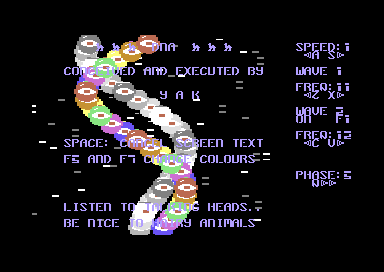
\includegraphics[width=10cm]{src/dna/dnascreenshot.png}%
\caption{DNA: A pause mode within a pause mode.}
\end{figure}

\begin{figure}[H]

    \centering
    \foreach \l in {1, ...,16}
    {
      \includegraphics[width=3cm]{dna/dna\l.png}%
    }%
    \foreach \l in {17, ...,24}
    {
      \includegraphics[width=4cm]{dna/dna\l.png}%
    }%
\caption{The first screen\index{screen} paint in DNA. There are 24 raster interrupts allowing us to paint a long chain of sprites\index{sprites}.}
\end{figure}
\clearpage

\begin{lstlisting}[caption=Defining the text for the DNA screen\index{screen},escapechar=\%]
titleTextLine1%\index{titleTextLine1}%   .TEXT "    % % %  DNA  % % %   "
titleTextLine2%\index{titleTextLine2}%   .TEXT " CONCEIVED%\index{CONCEIVED}% AND EXECUTED%\index{EXECUTED}% B"
titleTextLine3%\index{titleTextLine3}%   .TEXT "Y            Y A K       "
titleTextLine4%\index{titleTextLine4}%   .TEXT " SPACE: CANCEL SCREEN TEX"
titleTextLine5%\index{titleTextLine5}%   .TEXT "TF5 AND F7 CHANGE COLOURS"
titleTextLine6%\index{titleTextLine6}%   .TEXT " LISTEN TO TALKING%\index{TALKING}% HEADS."
titleTextLine7%\index{titleTextLine7}%   .TEXT ".BE NICE TO HAIRY ANIMALS%\index{ANIMALS}% "
\end{lstlisting}

Minter first shared it as a tiny 11K demo in a UK Compunet forum in the summer of 
1986. It followed shortly after 'Torus', an oscillator-based demo, shared at the same time and which we
cover elsewhere : both are sprite-based
light synthesisers where, like Psychedelia and Colorspace, the player gets to experiment with different
configurations that control the behaviour of a frantic assembly of brightly colored, pulsating sprites\index{sprites}.

DNA has an unapologetically daft premise: two chains of flashing eyeballs cascade down the
screen\index{screen} in an unsettling, blinking helix configuration. Your object as player is to twiddle the available
knobs to see if you can get them to do anything interesting while listening to your favorite music.

For its time DNA's most noteworthy feature was the number of sprites\index{sprites} being written to the screen\index{screen}. There are
48 eyeballs displayed at any one time, in addition to a pair of parallax\index{parallax} starfields drifting past in the
background\index{background}. As you may have gathered by now, the C64 can only support 8 sprites\index{sprites} in total so this would
have seemed like wizardry to the uninitiated. If you're not dipping into this chapter at random, but have
read any of the previous chapters in this book you may already be able to guess the secret to this 
unsettling feat: raster interrupts.

As elsewhere in Iridis Alpha the trick to filling the screen\index{screen} with sprites\index{sprites} is to write a tight piece of code
that can run periodically during a single paint of the screen\index{screen}, adding a layer of sprites\index{sprites} to each horizontal
section. We tell the C64 where we want the raster to interrupt\index{interrupt} its progress and call our code. This code
will then paint as many sprites\index{sprites} as possible on the horizontal layer. DNA takes the approach of painting a
pair of eyeballs at 8 pixel vertical intervals, so each horizontal layer is 8 pixels tall. 
These intervals are defined in \icode{dnaSpritesYPositionsArray\index{dnaSpritesYPositionsArray}}:

\begin{lstlisting}[escapechar=\%]
dnaSpritesYPositionsArray%\index{dnaSpritesYPositionsArray}%       .BYTE $30,$38,$40,$48,$50,$58,$60,$68
                                .BYTE $70,$78,$80,$88,$90,$98,$A0,$A8
                                .BYTE $B0,$B8,$C0,$C8,$D0,$D8,$E0,$E8
                                .BYTE END_SENTINEL%\index{END\_SENTINEL}%
\end{lstlisting}

While the Y co-ordinates of the sprites\index{sprites} are set in stone, their X co-ordinates must be calculated on the fly
and indeed the purpose of the twiddling knobs is to control the way these co-ordinates are generated. Initially
the X positions are all set to 192 (\$C0):

\begin{lstlisting}[escapechar=\%]
dnaSpritesXPositionsArray%\index{dnaSpritesXPositionsArray}%       .BYTE $C0,$C0,$C0,$C0,$C0,$C0,$C0,$C0
                                .BYTE $C0,$C0,$C0,$C0,$C0,$C0,$C0,$C0
                                .BYTE $C0,$C0,$C0,$C0,$C0,$C0,$C0,$C0
                                .BYTE $00,$00,$00,$00,$00,$00,$00,$00
                                .BYTE $00,$00,$00,$00,$00,$00,$00,$00
\end{lstlisting}

With every full paint of the screen\index{screen} calculates a new X co-ordinate and puts it at the head of the array. Depending
on the value given as the 'Speed' setting, it then shifts all the others in the array to the right by one position. 

\begin{lstlisting}[escapechar=\%]
DNA_PropagatePreviousXPosToTheRight%\index{DNA\_PropagatePreviousXPosToTheRight}%
        LDX #$27
PropagateToRightLoop%\index{PropagateToRightLoop}%   
        LDA dnaSpritesXPositionsArray%\index{dnaSpritesXPositionsArray}% - $01,X
        STA dnaSpritesXPositionsArray%\index{dnaSpritesXPositionsArray}%,X
        DEX
        BNE PropagateToRightLoop%\index{PropagateToRightLoop}%
        RTS
\end{lstlisting}

This very quickly fills the array.  We can see this in operation from the below
snippet in \icode{DNA\_MainAnimationRoutine}. In order to calculate the x position
for the right hand chain, it shows the value in
\icode{dnaCurrentPhase\index{dnaCurrentPhase}} being added to the value
\icode{dnaCurrent\-SpritesPosArrayIndex} to pick out a value in
\icode{dnaSpritesXPositionsArray\index{dnaSpritesXPositionsArray}} offset by the amount of the 'Phase' setting:

\begin{minipage}[b]{0.75\linewidth}
\centering
\begin{lstlisting}[caption=\icode{dnaCurrentPhase\index{dnaCurrentPhase}} is
set by the 'Q' key. ,basicstyle=\scriptsize\ttfamily,escapechar=\%]
  LDX dnaCurrentSpritesPosArrayIndex%\index{dnaCurrentSpritesPosArrayIndex}%
  ..
  ; Add in the phase to our index to the X position of the 
  ; sprite on the right hand chain. If the result is greater
  ; than the number of values in the array ($27) subtract it
  ; out again.
  TXA
  ..
  ADC dnaCurrentPhase%\index{dnaCurrentPhase}%
  CMP #$27
  BMI UpdateXPosWithPhase%\index{UpdateXPosWithPhase}%

  ; Back out the addition if result greater than $27.
  SEC
  SBC #$27
UpdateXPosWithPhase%\index{UpdateXPosWithPhase}%   
  ; Finally, use the offset given by the update value 
  ; in 'A', load it to 'X' and use it pick the X 
  ; position from dnaSpritesXPositionsArray%\index{dnaSpritesXPositionsArray}%.
  TAX
  LDA dnaSpritesXPositionsArray%\index{dnaSpritesXPositionsArray}%,X
  STA $D004,Y  ;Sprite 2 X Pos
\end{lstlisting}
\end{minipage}
\hspace{0.5cm}
\begin{minipage}[b]{0.25\linewidth}
\centering
      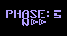
\includegraphics[width=3cm]{dna/dnaphase.png}%
      \vspace{2cm}
\end{minipage}
In essence, the 'Phase' setting  acts as an offset into the X
Position array picking up previous values of X Pos from the left hand
chain.

In the table below we've selected a few frames from the first second or two showing how the array fills up and how values from
the array are selected for the X position of the left and right chains. Notice how the 'Phase' setting of 5 effectively means
the right-hand chain lags 5 'eyeballs' behind the left chain in terms of the positions.

\begin{figure}[H]
{
  \setlength{\tabcolsep}{9.0pt}
  \setlength\cmidrulewidth{\heavyrulewidth} % Make cmidrule = 
    \begin{adjustbox}{center}
  \begin{tabular}{lcc}
  \toprule
    State & Left Chain & Right Chain \\
    \midrule
    \makecell[l]{
      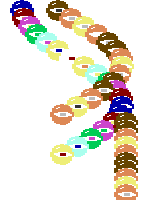
\includegraphics[height=2.5cm]{dna/initial/frame46.png}%
    } &
    \makecell[l]{
      \lstinputlisting[linewidth=4.5cm,framexleftmargin=-0.1cm,framexrightmargin=-0.22cm,
          basicstyle=\tiny\ttfamily,escapechar=!,backgroundcolor=\color{white},frame=single,framerule=0pt]{dna/initial/frame46.tex}
    } &
    \makecell[l]{
      \lstinputlisting[linewidth=4.5cm,framexleftmargin=-0.1cm,framexrightmargin=-0.22cm,
          basicstyle=\tiny\ttfamily,escapechar=!,backgroundcolor=\color{white},frame=single,framerule=0pt]{dna/initial/frame46r.tex}
    } \\
    \addlinespace
    \makecell[l]{
      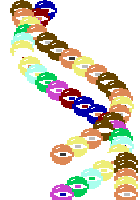
\includegraphics[height=2.5cm]{dna/initial/frame58.png}%
    } &
    \makecell[l]{
      \lstinputlisting[linewidth=4.5cm,framexleftmargin=-0.1cm,framexrightmargin=-0.22cm,
          basicstyle=\tiny\ttfamily,escapechar=!,backgroundcolor=\color{white},frame=single,framerule=0pt]{dna/initial/frame58.tex}
    } &
    \makecell[l]{
      \lstinputlisting[linewidth=4.5cm,framexleftmargin=-0.1cm,framexrightmargin=-0.22cm,
          basicstyle=\tiny\ttfamily,escapechar=!,backgroundcolor=\color{white},frame=single,framerule=0pt]{dna/initial/frame58r.tex}
    } \\
    \addlinespace
    \makecell[l]{
      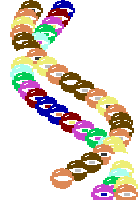
\includegraphics[height=2.5cm]{dna/initial/frame67.png}%
    } &
    \makecell[l]{
      \lstinputlisting[linewidth=4.5cm,framexleftmargin=-0.1cm,framexrightmargin=-0.22cm,
          basicstyle=\tiny\ttfamily,escapechar=!,backgroundcolor=\color{white},frame=single,framerule=0pt]{dna/initial/frame67.tex}
    } &
    \makecell[l]{
      \lstinputlisting[linewidth=4.5cm,framexleftmargin=-0.1cm,framexrightmargin=-0.22cm,
          basicstyle=\tiny\ttfamily,escapechar=!,backgroundcolor=\color{white},frame=single,framerule=0pt]{dna/initial/frame67r.tex}
    } \\
    \addlinespace
      \bottomrule
      \end{tabular}
    \end{adjustbox}
  }\caption{Examples of the x co-ordinates (highlighted) in \icode{dnaSpritesXPositionsArray\index{dnaSpritesXPositionsArray}} used by the left and right chain when 'phase' is set to 5.}
  \end{figure}

We said a new value for the top eye-ball in each chain is calculated every paint, but whether the existing
values get propagated to the right in \icode{dnaSpritesXPositionsArray\index{dnaSpritesXPositionsArray}} depends on the 'Speed' setting:

\begin{minipage}[b]{0.75\linewidth}
\centering
\begin{lstlisting}[caption=\icode{dnaCurrentSpeed\index{dnaCurrentSpeed}} is set by the 'A' and 'S' keys.,escapechar=\%]
UpdateXPosArrays%\index{UpdateXPosArrays}%
    DEC actualSpeed%\index{actualSpeed}%
    BNE CalculateNewXPosForHead%\index{CalculateNewXPosForHead}%

    ; The speed setting determines how quickly
    ; the X pos values are propagated down the chains.
    LDA dnaCurrentSpeed%\index{dnaCurrentSpeed}%
    STA actualSpeed%\index{actualSpeed}%
    JSR DNA_PropagatePreviousXPosToTheRight%\index{DNA\_PropagatePreviousXPosToTheRight}%
\end{lstlisting}
\end{minipage}
\hspace{0.5cm}
\begin{minipage}[b]{0.25\linewidth}
\centering
      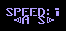
\includegraphics[width=3cm]{dna/dnaspeed.png}%
      \vspace{2cm}
\end{minipage}

The 'Speed' setting is effectively a counter that is decremented at every paint, once it reaches zero it gets reset back to 
its initial value (in this case '1') and the X Positions are all shifted to the right in \icode{dnaSpritesXPositionsArray\index{dnaSpritesXPositionsArray}}.

How is the new value for the eyeball at the head of each chain calculated? We get that it's updated at every screen\index{screen} paint
but what determines it? The calculation is a two-phase process but both phases depend on the same array of values stored
in \icode{newXPosOffsetsArray\index{newXPosOffsetsArray}}. This is a rattle-bag of X positions describing a more or less continuous curve:

\begin{lstlisting}[escapechar=\%,caption=Notice that the values start at \icode{\$40}\, rise gradually to \icode{\$80}\, back to \icode{\$00} and then
back up to \icode{\$40} again.]
newXPosOffsetsArray%\index{newXPosOffsetsArray}%  .BYTE $40,$46,$4C,$53,$58,$5E,$63,$68
                     .BYTE $6D,$71,$75,$78,$7B,$7D,$7E,$7F
                     .BYTE $80,$7F,$7E,$7D,$7B,$78,$75,$71
                     .BYTE $6D,$68,$63,$5E,$58,$52,$4C,$46
                     .BYTE $40,$39,$33,$2D,$27,$21,$1C,$17
                     .BYTE $12,$0E,$0A,$07,$04,$02,$01,$00
                     .BYTE $00,$00,$01,$02,$04,$07,$0A,$0E
                     .BYTE $12,$17,$1C,$21,$27,$2D,$33,$39
                     .BYTE END_SENTINEL%\index{END\_SENTINEL}%
\end{lstlisting}

The other factors in this calculation are the 'Frequency' selected for each chain, the left-hand chain (Wave 1) and the right-hand
chain (Wave 2). The values that do the most work are \icode{xPosOffsetForWave1\index{xPosOffsetForWave1}} and \icode{xPosOffsetForWave2\index{xPosOffsetForWave2}}. 

\begin{minipage}[b]{0.75\linewidth}
\centering
\begin{lstlisting}[caption=The value selected for 'Frequency' for Wave 1 and 2 translates to settings used in calculating the next X position for each chain.,escapechar=\%]
DNA_UpdateSettingsBasedOnFrequency%\index{DNA\_UpdateSettingsBasedOnFrequency}%
  LDA dnaWave1Frequency%\index{dnaWave1Frequency}%
  AND #$1F
  TAX
  LDA timesToNextUpdateForFrequency%\index{timesToNextUpdateForFrequency}%,X
  STA initialTimeToNextUpdateForWave1%\index{initialTimeToNextUpdateForWave1}%
  STA timeToNextUpdateCounterForWave1%\index{timeToNextUpdateCounterForWave1}%
  LDA xPosOffsetsForFrequency%\index{xPosOffsetsForFrequency}%,X
  STA xPosOffsetForWave1%\index{xPosOffsetForWave1}%

  LDA dnaWave2Frequency%\index{dnaWave2Frequency}%
  AND #$1F
  TAX
  LDA timesToNextUpdateForFrequency%\index{timesToNextUpdateForFrequency}%,X
  STA initialTimeToNextUpdateForWave2%\index{initialTimeToNextUpdateForWave2}%
  STA timeToNextUpdateCounterForWave2%\index{timeToNextUpdateCounterForWave2}%
  LDA xPosOffsetsForFrequency%\index{xPosOffsetsForFrequency}%,X
  STA xPosOffsetForWave2%\index{xPosOffsetForWave2}%
  JMP DNA_UpdateDisplayedSettings%\index{DNA\_UpdateDisplayedSettings}%
  ; Returns%\index{Returns}%
\end{lstlisting}
\end{minipage}
\hspace{0.5cm}
\begin{minipage}[b]{0.25\linewidth}
\centering
      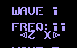
\includegraphics[width=3cm]{dna/dnafreq1.png}\\
      \vspace{1cm}
      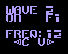
\includegraphics[width=3cm]{dna/dnafreq2.png}%
      \vspace{1cm}
\end{minipage}
As we can see above these are populated from \icode{xPosOffsetsForFrequency\index{xPosOffsetsForFrequency}} using the 'Frequency' as an index.

\begin{lstlisting}[escapechar=\%]
  ..
  LDA xPosOffsetsForFrequency%\index{xPosOffsetsForFrequency}%,X
  STA xPosOffsetForWave1%\index{xPosOffsetForWave1}%

  ..
  LDA xPosOffsetsForFrequency%\index{xPosOffsetsForFrequency}%,X
  STA xPosOffsetForWave2%\index{xPosOffsetForWave2}%
\end{lstlisting}

In each case the value populated here is added to a value selected from \icode{newXPosOffsetsArray\index{newXPosOffsetsArray}} to give the 
new X position for the eyeball at the head of the chain. Well, in a way that's only half true. Separate positions
are indeed calculated for the left and right chain, but at the end of the day the position calculate for the right-hand
chain (Wave 2) is purely notional. It's just used as an initial value that the value calculated for the left-hand chain
is layered on to. This allows the two chains to 'interfere' with each other, as though the position of one affects the
other - and reduces the chance of the two overlapping too much:

\begin{lstlisting}[caption=From \icode{CalculateValueOfNewXPosForWave1},escapechar=\%]
UpdateHeadOfWave%\index{UpdateHeadOfWave}%   
  ; Take the new X Pos value we calculated for Wave 2, add the position
  ; we calculated for Wave 1 and make that the new position for the lead
  ; sprite at the head of dnaSpritesXPositionsArray%\index{dnaSpritesXPositionsArray}%.
  LDA notionalNewXPosForWave2%\index{notionalNewXPosForWave2}%
  CLC
  ADC newXPosForWave1%\index{newXPosForWave1}%
  STA dnaSpritesXPositionsArray%\index{dnaSpritesXPositionsArray}%
\end{lstlisting}

When we compare the routines responsible for calculating the X Pos for Wave 2 and Wave 1 side by side on the next
page we can see many similarities between the two.

\begin{minipage}[b]{0.50\linewidth}
\centering
\begin{lstlisting}[escapechar=\%,basicstyle=\tiny\ttfamily, caption=Calculate a notional X Pos value for Wave 2. This routine\index{routine} is called by the one on the
right\, its return value is \icode{notionalNewXPosForWave2\index{notionalNewXPosForWave2}}. ]
CalculateValueOfNewXPosForWave2
  LDA dnaWave2Enabled%\index{dnaWave2Enabled}%
  BNE NewXPosWhenWave2Enabled%\index{NewXPosWhenWave2Enabled}%

  ; If wave 2 is not enabled set $40
  ; as the initial X Pos (it will be
  ; incremented later).
  LDA #XPOS_OFFSETS_ARRAY_SIZE%\index{XPOS\_OFFSETS\_ARRAY\_SIZE}%
  STA notionalNewXPosForWave2%\index{notionalNewXPosForWave2}%
ReturnFromNewXPos%\index{ReturnFromNewXPos}%   
  RTS

NewXPosWhenWave2Enabled%\index{NewXPosWhenWave2Enabled}%   
  DEC timeToNextUpdateCounterForWave2%\index{timeToNextUpdateCounterForWave2}%
  BNE ReturnFromNewXPos%\index{ReturnFromNewXPos}%

  LDA initialTimeToNextUpdateForWave2%\index{initialTimeToNextUpdateForWave2}%
  STA timeToNextUpdateCounterForWave2%\index{timeToNextUpdateCounterForWave2}%

  ; If right hand chain is enabled
  ; get value from newXPosOffsetsArray%\index{newXPosOffsetsArray}%,
  ; which has $40 (64) potential values. 
  ; This logic uses 
  ; indexToXPosDataArrayForWave2%\index{indexToXPosDataArrayForWave2}% 
  ; to get a value from it, halves it
  ; with ROR, and adds $40.
  LDX indexToXPosDataArrayForWave2%\index{indexToXPosDataArrayForWave2}%
  LDA newXPosOffsetsArray%\index{newXPosOffsetsArray}%,X
  CLC
  ROR         ; Halve it.
  CLC
  ADC #XPOS_OFFSETS_ARRAY_SIZE%\index{XPOS\_OFFSETS\_ARRAY\_SIZE}%
  STA notionalNewXPosForWave2%\index{notionalNewXPosForWave2}%

  ; Add xPosOffsetForWave2%\index{xPosOffsetForWave2}% to
  ; indexToXPosDataArrayForWave2%\index{indexToXPosDataArrayForWave2}%.
  ; Ensure it loops to start of array if
  ; greater than $40. 
  TXA
  CLC
  ADC xPosOffsetForWave2%\index{xPosOffsetForWave2}%
  CMP #XPOS_OFFSETS_ARRAY_SIZE%\index{XPOS\_OFFSETS\_ARRAY\_SIZE}%
  BMI NoLoopingRequired%\index{NoLoopingRequired}%

  SEC
  SBC #XPOS_OFFSETS_ARRAY_SIZE%\index{XPOS\_OFFSETS\_ARRAY\_SIZE}%
NoLoopingRequired%\index{NoLoopingRequired}%   
  STA indexToXPosDataArrayForWave2%\index{indexToXPosDataArrayForWave2}%
  RTS
\end{lstlisting}
\end{minipage}
\hspace{0.5cm}
\begin{minipage}[b]{0.50\linewidth}
\centering
  \begin{lstlisting}[escapechar=\%,basicstyle=\tiny\ttfamily, caption=Calculate the new X Pos value for the head sprites\index{sprites}\, as well as propagate the
  values in \icode{dnaXPosDataHeadArray} to the right when required.]
CalculateValueOfNewXPosForWave1
  DEC actualSpeed%\index{actualSpeed}%
  BNE CalculateNewXPosForHead%\index{CalculateNewXPosForHead}%

  ; The speed setting determines how quickly 
  ; the X pos values are propagated down the chains.
  LDA dnaCurrentSpeed%\index{dnaCurrentSpeed}%
  STA actualSpeed%\index{actualSpeed}%
  JSR DNA_PropagatePreviousXPosToTheRight%\index{DNA\_PropagatePreviousXPosToTheRight}%
CalculateNewXPosForHead%\index{CalculateNewXPosForHead}%   
  ; Get a new value for Wave 2.
  JSR CalculateValueOfNewXPosForWave2
  DEC timeToNextUpdateCounterForWave1%\index{timeToNextUpdateCounterForWave1}%
  BNE ReturnFromUpdatingHead%\index{ReturnFromUpdatingHead}%

  LDA initialTimeToNextUpdateForWave1%\index{initialTimeToNextUpdateForWave1}%
  STA timeToNextUpdateCounterForWave1%\index{timeToNextUpdateCounterForWave1}%

  ; Get newXPosForWave1%\index{newXPosForWave1}%, this will be added to
  ; notionalNewXPosForWave2%\index{notionalNewXPosForWave2}%. Both are sourced
  ; from the same array newXPosOffsetsArray%\index{newXPosOffsetsArray}%.
  LDX indexToNextXPosForHead%\index{indexToNextXPosForHead}%
  LDA newXPosOffsetsArray%\index{newXPosOffsetsArray}%,X
  STA newXPosForWave1%\index{newXPosForWave1}%

  LDY dnaWave2Enabled%\index{dnaWave2Enabled}%
  BEQ UpdateHeadOfWave%\index{UpdateHeadOfWave}%

  ; Halve the offset we will use if
  ; the right hand chain is enabled.
  CLC
  ROR 
  STA newXPosForWave1%\index{newXPosForWave1}%
UpdateHeadOfWave%\index{UpdateHeadOfWave}%   
  ; Take the new X Pos value we calculated for Wave 2,
  ; add the position we calculated for Wave 1 and 
  ; make that the new position for the lead
  ; sprite at the head of dnaSpritesXPositionsArray%\index{dnaSpritesXPositionsArray}%.
  LDA notionalNewXPosForWave2%\index{notionalNewXPosForWave2}%
  CLC
  ADC newXPosForWave1%\index{newXPosForWave1}%
  STA dnaSpritesXPositionsArray%\index{dnaSpritesXPositionsArray}%

  ; Get value for indexToNextXPosForHead%\index{indexToNextXPosForHead}% for the next
  ; time around. Ensure it loops to start of array if 
  ; greater than $40.
  TXA
  CLC
  ADC xPosOffsetForWave1%\index{xPosOffsetForWave1}%
  TAX
  CPX #XPOS_OFFSETS_ARRAY_SIZE%\index{XPOS\_OFFSETS\_ARRAY\_SIZE}%
  BMI UpdateNextXPos%\index{UpdateNextXPos}%

  SEC
  SBC #XPOS_OFFSETS_ARRAY_SIZE%\index{XPOS\_OFFSETS\_ARRAY\_SIZE}%
  TAX
UpdateNextXPos%\index{UpdateNextXPos}%   
  STX indexToNextXPosForHead%\index{indexToNextXPosForHead}%
ReturnFromUpdatingHead%\index{ReturnFromUpdatingHead}%   
  RTS
\end{lstlisting}
\end{minipage}


They are both maintaining and updating an index into 
\icode{newXPosOffsetsArray\index{newXPosOffsetsArray}} and using that to come up with a new X position. They both have to deal towards the end
of the routine\index{routine} with the need to ensure the index does not exceed \icode{\$40} and subtract \icode{\$40} from it if
it does. The output of \icode{CalculateValueOfNewXPosForWave2} is essentially the value stored in \icode{notionalNewXPosForWave2\index{notionalNewXPosForWave2}}
and this is what is used as the input above, in conjunction with \icode{newXPosForWave1\index{newXPosForWave1}}, to come up with the final
value for the X position for Wave 1. It is this value that gets added to the head of the working array \icode{dnaXPosDataHeadArray}
by \icode{DNA\_PropagatePreviousXPosToTheRight}.







\begin{figure}[H]
  {
    \setlength{\tabcolsep}{1.0pt}
    \setlength\cmidrulewidth{\heavyrulewidth} % Make cmidrule = 
    \begin{adjustbox}{width=14cm,center}
      \begin{tabular}{ccc}
        \toprule
        Sprite0 & Sprite1 & Sprite2 \\
        \midrule
\makecell[l]{
	\begin{subfigure}{0.3\textwidth}
    \def\MULTICOLORONE{red}
    \def\MULTICOLORTWO{white}
    \def\SPRITECOLOR{yellow}
		
\begin{figure}[H]
  {
    \setlength{\tabcolsep}{3.0pt}
    \setlength\cmidrulewidth{\heavyrulewidth} % Make cmidrule = 
    \begin{adjustbox}{width=3cm,center}
      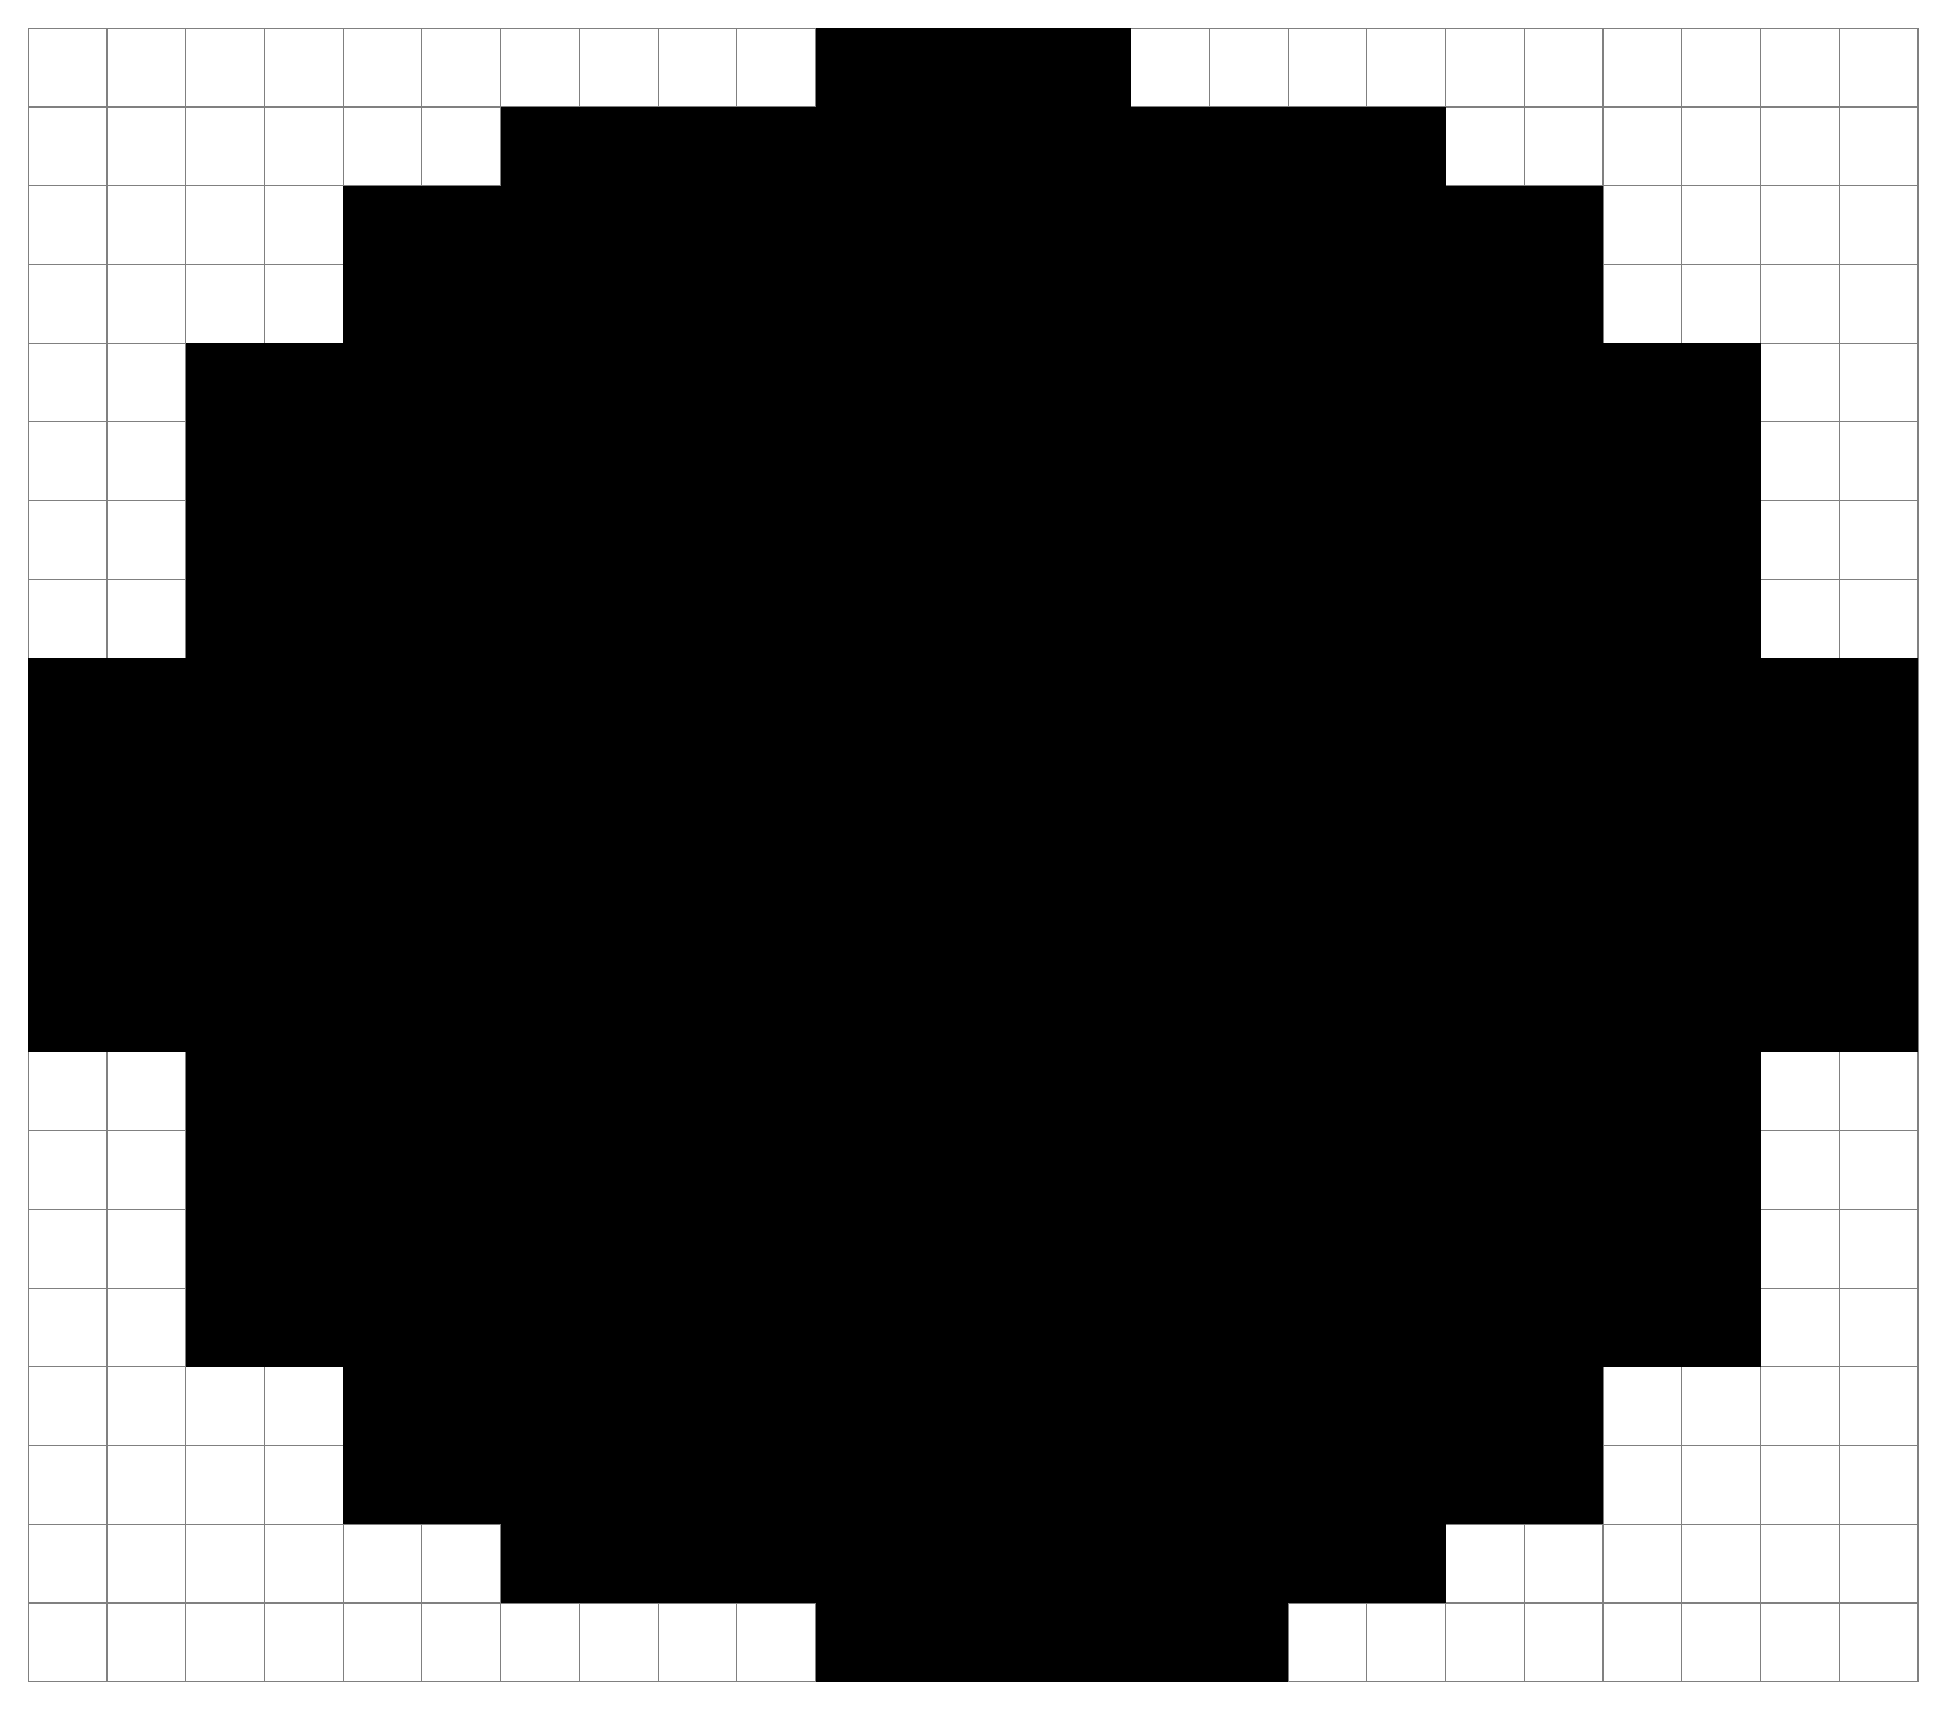
\begin{tikzpicture}

	\draw[step=1.0,gray,thin] (0,0) grid (24,21);
	\fill[\SPRITECOLOR] (10,20) rectangle ++ (1,1);
	\fill[\SPRITECOLOR] (11,20) rectangle ++ (1,1);
	\fill[\SPRITECOLOR] (12,20) rectangle ++ (1,1);
	\fill[\SPRITECOLOR] (13,20) rectangle ++ (1,1);
	\fill[\SPRITECOLOR] (6,19) rectangle ++ (1,1);
	\fill[\SPRITECOLOR] (7,19) rectangle ++ (1,1);
	\fill[\SPRITECOLOR] (8,19) rectangle ++ (1,1);
	\fill[\SPRITECOLOR] (9,19) rectangle ++ (1,1);
	\fill[\SPRITECOLOR] (10,19) rectangle ++ (1,1);
	\fill[\SPRITECOLOR] (11,19) rectangle ++ (1,1);
	\fill[\SPRITECOLOR] (12,19) rectangle ++ (1,1);
	\fill[\SPRITECOLOR] (13,19) rectangle ++ (1,1);
	\fill[\SPRITECOLOR] (14,19) rectangle ++ (1,1);
	\fill[\SPRITECOLOR] (15,19) rectangle ++ (1,1);
	\fill[\SPRITECOLOR] (16,19) rectangle ++ (1,1);
	\fill[\SPRITECOLOR] (17,19) rectangle ++ (1,1);
	\fill[\SPRITECOLOR] (4,18) rectangle ++ (1,1);
	\fill[\SPRITECOLOR] (5,18) rectangle ++ (1,1);
	\fill[\SPRITECOLOR] (6,18) rectangle ++ (1,1);
	\fill[\SPRITECOLOR] (7,18) rectangle ++ (1,1);
	\fill[\SPRITECOLOR] (8,18) rectangle ++ (1,1);
	\fill[\SPRITECOLOR] (9,18) rectangle ++ (1,1);
	\fill[\SPRITECOLOR] (10,18) rectangle ++ (1,1);
	\fill[\SPRITECOLOR] (11,18) rectangle ++ (1,1);
	\fill[\SPRITECOLOR] (12,18) rectangle ++ (1,1);
	\fill[\SPRITECOLOR] (13,18) rectangle ++ (1,1);
	\fill[\SPRITECOLOR] (14,18) rectangle ++ (1,1);
	\fill[\SPRITECOLOR] (15,18) rectangle ++ (1,1);
	\fill[\SPRITECOLOR] (16,18) rectangle ++ (1,1);
	\fill[\SPRITECOLOR] (17,18) rectangle ++ (1,1);
	\fill[\SPRITECOLOR] (18,18) rectangle ++ (1,1);
	\fill[\SPRITECOLOR] (19,18) rectangle ++ (1,1);
	\fill[\SPRITECOLOR] (4,17) rectangle ++ (1,1);
	\fill[\SPRITECOLOR] (5,17) rectangle ++ (1,1);
	\fill[\SPRITECOLOR] (6,17) rectangle ++ (1,1);
	\fill[\SPRITECOLOR] (7,17) rectangle ++ (1,1);
	\fill[\MULTICOLORTWO] (8,17) rectangle ++ (1,1);
	\fill[\MULTICOLORTWO] (9,17) rectangle ++ (1,1);
	\fill[\SPRITECOLOR] (10,17) rectangle ++ (1,1);
	\fill[\SPRITECOLOR] (11,17) rectangle ++ (1,1);
	\fill[\SPRITECOLOR] (12,17) rectangle ++ (1,1);
	\fill[\SPRITECOLOR] (13,17) rectangle ++ (1,1);
	\fill[\SPRITECOLOR] (14,17) rectangle ++ (1,1);
	\fill[\SPRITECOLOR] (15,17) rectangle ++ (1,1);
	\fill[\SPRITECOLOR] (16,17) rectangle ++ (1,1);
	\fill[\SPRITECOLOR] (17,17) rectangle ++ (1,1);
	\fill[\SPRITECOLOR] (18,17) rectangle ++ (1,1);
	\fill[\SPRITECOLOR] (19,17) rectangle ++ (1,1);
	\fill[\SPRITECOLOR] (2,16) rectangle ++ (1,1);
	\fill[\SPRITECOLOR] (3,16) rectangle ++ (1,1);
	\fill[\SPRITECOLOR] (4,16) rectangle ++ (1,1);
	\fill[\SPRITECOLOR] (5,16) rectangle ++ (1,1);
	\fill[\MULTICOLORTWO] (6,16) rectangle ++ (1,1);
	\fill[\MULTICOLORTWO] (7,16) rectangle ++ (1,1);
	\fill[\SPRITECOLOR] (8,16) rectangle ++ (1,1);
	\fill[\SPRITECOLOR] (9,16) rectangle ++ (1,1);
	\fill[\SPRITECOLOR] (10,16) rectangle ++ (1,1);
	\fill[\SPRITECOLOR] (11,16) rectangle ++ (1,1);
	\fill[\SPRITECOLOR] (12,16) rectangle ++ (1,1);
	\fill[\SPRITECOLOR] (13,16) rectangle ++ (1,1);
	\fill[\SPRITECOLOR] (14,16) rectangle ++ (1,1);
	\fill[\SPRITECOLOR] (15,16) rectangle ++ (1,1);
	\fill[\SPRITECOLOR] (16,16) rectangle ++ (1,1);
	\fill[\SPRITECOLOR] (17,16) rectangle ++ (1,1);
	\fill[\SPRITECOLOR] (18,16) rectangle ++ (1,1);
	\fill[\SPRITECOLOR] (19,16) rectangle ++ (1,1);
	\fill[\SPRITECOLOR] (20,16) rectangle ++ (1,1);
	\fill[\SPRITECOLOR] (21,16) rectangle ++ (1,1);
	\fill[\SPRITECOLOR] (2,15) rectangle ++ (1,1);
	\fill[\SPRITECOLOR] (3,15) rectangle ++ (1,1);
	\fill[\SPRITECOLOR] (4,15) rectangle ++ (1,1);
	\fill[\SPRITECOLOR] (5,15) rectangle ++ (1,1);
	\fill[\SPRITECOLOR] (6,15) rectangle ++ (1,1);
	\fill[\SPRITECOLOR] (7,15) rectangle ++ (1,1);
	\fill[\SPRITECOLOR] (8,15) rectangle ++ (1,1);
	\fill[\SPRITECOLOR] (9,15) rectangle ++ (1,1);
	\fill[\SPRITECOLOR] (10,15) rectangle ++ (1,1);
	\fill[\SPRITECOLOR] (11,15) rectangle ++ (1,1);
	\fill[\SPRITECOLOR] (12,15) rectangle ++ (1,1);
	\fill[\SPRITECOLOR] (13,15) rectangle ++ (1,1);
	\fill[\SPRITECOLOR] (14,15) rectangle ++ (1,1);
	\fill[\SPRITECOLOR] (15,15) rectangle ++ (1,1);
	\fill[\SPRITECOLOR] (16,15) rectangle ++ (1,1);
	\fill[\SPRITECOLOR] (17,15) rectangle ++ (1,1);
	\fill[\SPRITECOLOR] (18,15) rectangle ++ (1,1);
	\fill[\SPRITECOLOR] (19,15) rectangle ++ (1,1);
	\fill[\SPRITECOLOR] (20,15) rectangle ++ (1,1);
	\fill[\SPRITECOLOR] (21,15) rectangle ++ (1,1);
	\fill[\SPRITECOLOR] (2,14) rectangle ++ (1,1);
	\fill[\SPRITECOLOR] (3,14) rectangle ++ (1,1);
	\fill[\SPRITECOLOR] (4,14) rectangle ++ (1,1);
	\fill[\SPRITECOLOR] (5,14) rectangle ++ (1,1);
	\fill[\SPRITECOLOR] (6,14) rectangle ++ (1,1);
	\fill[\SPRITECOLOR] (7,14) rectangle ++ (1,1);
	\fill[\SPRITECOLOR] (8,14) rectangle ++ (1,1);
	\fill[\SPRITECOLOR] (9,14) rectangle ++ (1,1);
	\fill[\SPRITECOLOR] (10,14) rectangle ++ (1,1);
	\fill[\SPRITECOLOR] (11,14) rectangle ++ (1,1);
	\fill[\SPRITECOLOR] (12,14) rectangle ++ (1,1);
	\fill[\SPRITECOLOR] (13,14) rectangle ++ (1,1);
	\fill[\SPRITECOLOR] (14,14) rectangle ++ (1,1);
	\fill[\SPRITECOLOR] (15,14) rectangle ++ (1,1);
	\fill[\SPRITECOLOR] (16,14) rectangle ++ (1,1);
	\fill[\SPRITECOLOR] (17,14) rectangle ++ (1,1);
	\fill[\SPRITECOLOR] (18,14) rectangle ++ (1,1);
	\fill[\SPRITECOLOR] (19,14) rectangle ++ (1,1);
	\fill[\SPRITECOLOR] (20,14) rectangle ++ (1,1);
	\fill[\SPRITECOLOR] (21,14) rectangle ++ (1,1);
	\fill[\SPRITECOLOR] (2,13) rectangle ++ (1,1);
	\fill[\SPRITECOLOR] (3,13) rectangle ++ (1,1);
	\fill[\SPRITECOLOR] (4,13) rectangle ++ (1,1);
	\fill[\SPRITECOLOR] (5,13) rectangle ++ (1,1);
	\fill[\SPRITECOLOR] (6,13) rectangle ++ (1,1);
	\fill[\SPRITECOLOR] (7,13) rectangle ++ (1,1);
	\fill[\MULTICOLORTWO] (8,13) rectangle ++ (1,1);
	\fill[\MULTICOLORTWO] (9,13) rectangle ++ (1,1);
	\fill[\MULTICOLORTWO] (10,13) rectangle ++ (1,1);
	\fill[\MULTICOLORTWO] (11,13) rectangle ++ (1,1);
	\fill[\MULTICOLORTWO] (12,13) rectangle ++ (1,1);
	\fill[\MULTICOLORTWO] (13,13) rectangle ++ (1,1);
	\fill[\MULTICOLORTWO] (14,13) rectangle ++ (1,1);
	\fill[\MULTICOLORTWO] (15,13) rectangle ++ (1,1);
	\fill[\SPRITECOLOR] (16,13) rectangle ++ (1,1);
	\fill[\SPRITECOLOR] (17,13) rectangle ++ (1,1);
	\fill[\SPRITECOLOR] (18,13) rectangle ++ (1,1);
	\fill[\SPRITECOLOR] (19,13) rectangle ++ (1,1);
	\fill[\SPRITECOLOR] (20,13) rectangle ++ (1,1);
	\fill[\SPRITECOLOR] (21,13) rectangle ++ (1,1);
	\fill[\SPRITECOLOR] (0,12) rectangle ++ (1,1);
	\fill[\SPRITECOLOR] (1,12) rectangle ++ (1,1);
	\fill[\SPRITECOLOR] (2,12) rectangle ++ (1,1);
	\fill[\SPRITECOLOR] (3,12) rectangle ++ (1,1);
	\fill[\SPRITECOLOR] (4,12) rectangle ++ (1,1);
	\fill[\SPRITECOLOR] (5,12) rectangle ++ (1,1);
	\fill[\MULTICOLORTWO] (6,12) rectangle ++ (1,1);
	\fill[\MULTICOLORTWO] (7,12) rectangle ++ (1,1);
	\fill[\MULTICOLORTWO] (8,12) rectangle ++ (1,1);
	\fill[\MULTICOLORTWO] (9,12) rectangle ++ (1,1);
	\fill[\MULTICOLORTWO] (10,12) rectangle ++ (1,1);
	\fill[\MULTICOLORTWO] (11,12) rectangle ++ (1,1);
	\fill[\MULTICOLORTWO] (12,12) rectangle ++ (1,1);
	\fill[\MULTICOLORTWO] (13,12) rectangle ++ (1,1);
	\fill[\MULTICOLORTWO] (14,12) rectangle ++ (1,1);
	\fill[\MULTICOLORTWO] (15,12) rectangle ++ (1,1);
	\fill[\MULTICOLORTWO] (16,12) rectangle ++ (1,1);
	\fill[\MULTICOLORTWO] (17,12) rectangle ++ (1,1);
	\fill[\SPRITECOLOR] (18,12) rectangle ++ (1,1);
	\fill[\SPRITECOLOR] (19,12) rectangle ++ (1,1);
	\fill[\SPRITECOLOR] (20,12) rectangle ++ (1,1);
	\fill[\SPRITECOLOR] (21,12) rectangle ++ (1,1);
	\fill[\SPRITECOLOR] (22,12) rectangle ++ (1,1);
	\fill[\SPRITECOLOR] (23,12) rectangle ++ (1,1);
	\fill[\SPRITECOLOR] (0,11) rectangle ++ (1,1);
	\fill[\SPRITECOLOR] (1,11) rectangle ++ (1,1);
	\fill[\SPRITECOLOR] (2,11) rectangle ++ (1,1);
	\fill[\SPRITECOLOR] (3,11) rectangle ++ (1,1);
	\fill[\MULTICOLORTWO] (4,11) rectangle ++ (1,1);
	\fill[\MULTICOLORTWO] (5,11) rectangle ++ (1,1);
	\fill[\MULTICOLORTWO] (6,11) rectangle ++ (1,1);
	\fill[\MULTICOLORTWO] (7,11) rectangle ++ (1,1);
	\fill[\MULTICOLORTWO] (8,11) rectangle ++ (1,1);
	\fill[\MULTICOLORTWO] (9,11) rectangle ++ (1,1);
	\fill[\MULTICOLORONE] (10,11) rectangle ++ (1,1);
	\fill[\MULTICOLORONE] (11,11) rectangle ++ (1,1);
	\fill[\MULTICOLORONE] (12,11) rectangle ++ (1,1);
	\fill[\MULTICOLORONE] (13,11) rectangle ++ (1,1);
	\fill[\MULTICOLORONE] (14,11) rectangle ++ (1,1);
	\fill[\MULTICOLORONE] (15,11) rectangle ++ (1,1);
	\fill[\MULTICOLORTWO] (16,11) rectangle ++ (1,1);
	\fill[\MULTICOLORTWO] (17,11) rectangle ++ (1,1);
	\fill[\MULTICOLORTWO] (18,11) rectangle ++ (1,1);
	\fill[\MULTICOLORTWO] (19,11) rectangle ++ (1,1);
	\fill[\SPRITECOLOR] (20,11) rectangle ++ (1,1);
	\fill[\SPRITECOLOR] (21,11) rectangle ++ (1,1);
	\fill[\SPRITECOLOR] (22,11) rectangle ++ (1,1);
	\fill[\SPRITECOLOR] (23,11) rectangle ++ (1,1);
	\fill[\SPRITECOLOR] (0,10) rectangle ++ (1,1);
	\fill[\SPRITECOLOR] (1,10) rectangle ++ (1,1);
	\fill[\SPRITECOLOR] (2,10) rectangle ++ (1,1);
	\fill[\SPRITECOLOR] (3,10) rectangle ++ (1,1);
	\fill[\MULTICOLORTWO] (4,10) rectangle ++ (1,1);
	\fill[\MULTICOLORTWO] (5,10) rectangle ++ (1,1);
	\fill[\MULTICOLORTWO] (6,10) rectangle ++ (1,1);
	\fill[\MULTICOLORTWO] (7,10) rectangle ++ (1,1);
	\fill[\MULTICOLORTWO] (8,10) rectangle ++ (1,1);
	\fill[\MULTICOLORTWO] (9,10) rectangle ++ (1,1);
	\fill[\MULTICOLORONE] (10,10) rectangle ++ (1,1);
	\fill[\MULTICOLORONE] (11,10) rectangle ++ (1,1);
	\fill[\MULTICOLORONE] (12,10) rectangle ++ (1,1);
	\fill[\MULTICOLORONE] (13,10) rectangle ++ (1,1);
	\fill[\MULTICOLORONE] (14,10) rectangle ++ (1,1);
	\fill[\MULTICOLORONE] (15,10) rectangle ++ (1,1);
	\fill[\MULTICOLORTWO] (16,10) rectangle ++ (1,1);
	\fill[\MULTICOLORTWO] (17,10) rectangle ++ (1,1);
	\fill[\MULTICOLORTWO] (18,10) rectangle ++ (1,1);
	\fill[\MULTICOLORTWO] (19,10) rectangle ++ (1,1);
	\fill[\MULTICOLORTWO] (20,10) rectangle ++ (1,1);
	\fill[\MULTICOLORTWO] (21,10) rectangle ++ (1,1);
	\fill[\SPRITECOLOR] (22,10) rectangle ++ (1,1);
	\fill[\SPRITECOLOR] (23,10) rectangle ++ (1,1);
	\fill[\SPRITECOLOR] (0,9) rectangle ++ (1,1);
	\fill[\SPRITECOLOR] (1,9) rectangle ++ (1,1);
	\fill[\SPRITECOLOR] (2,9) rectangle ++ (1,1);
	\fill[\SPRITECOLOR] (3,9) rectangle ++ (1,1);
	\fill[\MULTICOLORTWO] (4,9) rectangle ++ (1,1);
	\fill[\MULTICOLORTWO] (5,9) rectangle ++ (1,1);
	\fill[\MULTICOLORTWO] (6,9) rectangle ++ (1,1);
	\fill[\MULTICOLORTWO] (7,9) rectangle ++ (1,1);
	\fill[\MULTICOLORTWO] (8,9) rectangle ++ (1,1);
	\fill[\MULTICOLORTWO] (9,9) rectangle ++ (1,1);
	\fill[\MULTICOLORONE] (10,9) rectangle ++ (1,1);
	\fill[\MULTICOLORONE] (11,9) rectangle ++ (1,1);
	\fill[\MULTICOLORONE] (12,9) rectangle ++ (1,1);
	\fill[\MULTICOLORONE] (13,9) rectangle ++ (1,1);
	\fill[\MULTICOLORONE] (14,9) rectangle ++ (1,1);
	\fill[\MULTICOLORONE] (15,9) rectangle ++ (1,1);
	\fill[\MULTICOLORTWO] (16,9) rectangle ++ (1,1);
	\fill[\MULTICOLORTWO] (17,9) rectangle ++ (1,1);
	\fill[\MULTICOLORTWO] (18,9) rectangle ++ (1,1);
	\fill[\MULTICOLORTWO] (19,9) rectangle ++ (1,1);
	\fill[\MULTICOLORTWO] (20,9) rectangle ++ (1,1);
	\fill[\MULTICOLORTWO] (21,9) rectangle ++ (1,1);
	\fill[\SPRITECOLOR] (22,9) rectangle ++ (1,1);
	\fill[\SPRITECOLOR] (23,9) rectangle ++ (1,1);
	\fill[\SPRITECOLOR] (0,8) rectangle ++ (1,1);
	\fill[\SPRITECOLOR] (1,8) rectangle ++ (1,1);
	\fill[\SPRITECOLOR] (2,8) rectangle ++ (1,1);
	\fill[\SPRITECOLOR] (3,8) rectangle ++ (1,1);
	\fill[\SPRITECOLOR] (4,8) rectangle ++ (1,1);
	\fill[\SPRITECOLOR] (5,8) rectangle ++ (1,1);
	\fill[\MULTICOLORTWO] (6,8) rectangle ++ (1,1);
	\fill[\MULTICOLORTWO] (7,8) rectangle ++ (1,1);
	\fill[\MULTICOLORTWO] (8,8) rectangle ++ (1,1);
	\fill[\MULTICOLORTWO] (9,8) rectangle ++ (1,1);
	\fill[\MULTICOLORTWO] (10,8) rectangle ++ (1,1);
	\fill[\MULTICOLORTWO] (11,8) rectangle ++ (1,1);
	\fill[\MULTICOLORTWO] (12,8) rectangle ++ (1,1);
	\fill[\MULTICOLORTWO] (13,8) rectangle ++ (1,1);
	\fill[\MULTICOLORTWO] (14,8) rectangle ++ (1,1);
	\fill[\MULTICOLORTWO] (15,8) rectangle ++ (1,1);
	\fill[\MULTICOLORTWO] (16,8) rectangle ++ (1,1);
	\fill[\MULTICOLORTWO] (17,8) rectangle ++ (1,1);
	\fill[\MULTICOLORTWO] (18,8) rectangle ++ (1,1);
	\fill[\MULTICOLORTWO] (19,8) rectangle ++ (1,1);
	\fill[\SPRITECOLOR] (20,8) rectangle ++ (1,1);
	\fill[\SPRITECOLOR] (21,8) rectangle ++ (1,1);
	\fill[\SPRITECOLOR] (22,8) rectangle ++ (1,1);
	\fill[\SPRITECOLOR] (23,8) rectangle ++ (1,1);
	\fill[\SPRITECOLOR] (2,7) rectangle ++ (1,1);
	\fill[\SPRITECOLOR] (3,7) rectangle ++ (1,1);
	\fill[\SPRITECOLOR] (4,7) rectangle ++ (1,1);
	\fill[\SPRITECOLOR] (5,7) rectangle ++ (1,1);
	\fill[\SPRITECOLOR] (6,7) rectangle ++ (1,1);
	\fill[\SPRITECOLOR] (7,7) rectangle ++ (1,1);
	\fill[\SPRITECOLOR] (8,7) rectangle ++ (1,1);
	\fill[\SPRITECOLOR] (9,7) rectangle ++ (1,1);
	\fill[\MULTICOLORTWO] (10,7) rectangle ++ (1,1);
	\fill[\MULTICOLORTWO] (11,7) rectangle ++ (1,1);
	\fill[\MULTICOLORTWO] (12,7) rectangle ++ (1,1);
	\fill[\MULTICOLORTWO] (13,7) rectangle ++ (1,1);
	\fill[\MULTICOLORTWO] (14,7) rectangle ++ (1,1);
	\fill[\MULTICOLORTWO] (15,7) rectangle ++ (1,1);
	\fill[\SPRITECOLOR] (16,7) rectangle ++ (1,1);
	\fill[\SPRITECOLOR] (17,7) rectangle ++ (1,1);
	\fill[\SPRITECOLOR] (18,7) rectangle ++ (1,1);
	\fill[\SPRITECOLOR] (19,7) rectangle ++ (1,1);
	\fill[\SPRITECOLOR] (20,7) rectangle ++ (1,1);
	\fill[\SPRITECOLOR] (21,7) rectangle ++ (1,1);
	\fill[\SPRITECOLOR] (2,6) rectangle ++ (1,1);
	\fill[\SPRITECOLOR] (3,6) rectangle ++ (1,1);
	\fill[\SPRITECOLOR] (4,6) rectangle ++ (1,1);
	\fill[\SPRITECOLOR] (5,6) rectangle ++ (1,1);
	\fill[\SPRITECOLOR] (6,6) rectangle ++ (1,1);
	\fill[\SPRITECOLOR] (7,6) rectangle ++ (1,1);
	\fill[\SPRITECOLOR] (8,6) rectangle ++ (1,1);
	\fill[\SPRITECOLOR] (9,6) rectangle ++ (1,1);
	\fill[\SPRITECOLOR] (10,6) rectangle ++ (1,1);
	\fill[\SPRITECOLOR] (11,6) rectangle ++ (1,1);
	\fill[\SPRITECOLOR] (12,6) rectangle ++ (1,1);
	\fill[\SPRITECOLOR] (13,6) rectangle ++ (1,1);
	\fill[\SPRITECOLOR] (14,6) rectangle ++ (1,1);
	\fill[\SPRITECOLOR] (15,6) rectangle ++ (1,1);
	\fill[\SPRITECOLOR] (16,6) rectangle ++ (1,1);
	\fill[\SPRITECOLOR] (17,6) rectangle ++ (1,1);
	\fill[\SPRITECOLOR] (18,6) rectangle ++ (1,1);
	\fill[\SPRITECOLOR] (19,6) rectangle ++ (1,1);
	\fill[\SPRITECOLOR] (20,6) rectangle ++ (1,1);
	\fill[\SPRITECOLOR] (21,6) rectangle ++ (1,1);
	\fill[\SPRITECOLOR] (2,5) rectangle ++ (1,1);
	\fill[\SPRITECOLOR] (3,5) rectangle ++ (1,1);
	\fill[\SPRITECOLOR] (4,5) rectangle ++ (1,1);
	\fill[\SPRITECOLOR] (5,5) rectangle ++ (1,1);
	\fill[\SPRITECOLOR] (6,5) rectangle ++ (1,1);
	\fill[\SPRITECOLOR] (7,5) rectangle ++ (1,1);
	\fill[\SPRITECOLOR] (8,5) rectangle ++ (1,1);
	\fill[\SPRITECOLOR] (9,5) rectangle ++ (1,1);
	\fill[\SPRITECOLOR] (10,5) rectangle ++ (1,1);
	\fill[\SPRITECOLOR] (11,5) rectangle ++ (1,1);
	\fill[\SPRITECOLOR] (12,5) rectangle ++ (1,1);
	\fill[\SPRITECOLOR] (13,5) rectangle ++ (1,1);
	\fill[\SPRITECOLOR] (14,5) rectangle ++ (1,1);
	\fill[\SPRITECOLOR] (15,5) rectangle ++ (1,1);
	\fill[\SPRITECOLOR] (16,5) rectangle ++ (1,1);
	\fill[\SPRITECOLOR] (17,5) rectangle ++ (1,1);
	\fill[\SPRITECOLOR] (18,5) rectangle ++ (1,1);
	\fill[\SPRITECOLOR] (19,5) rectangle ++ (1,1);
	\fill[\SPRITECOLOR] (20,5) rectangle ++ (1,1);
	\fill[\SPRITECOLOR] (21,5) rectangle ++ (1,1);
	\fill[\SPRITECOLOR] (2,4) rectangle ++ (1,1);
	\fill[\SPRITECOLOR] (3,4) rectangle ++ (1,1);
	\fill[\SPRITECOLOR] (4,4) rectangle ++ (1,1);
	\fill[\SPRITECOLOR] (5,4) rectangle ++ (1,1);
	\fill[\SPRITECOLOR] (6,4) rectangle ++ (1,1);
	\fill[\SPRITECOLOR] (7,4) rectangle ++ (1,1);
	\fill[\SPRITECOLOR] (8,4) rectangle ++ (1,1);
	\fill[\SPRITECOLOR] (9,4) rectangle ++ (1,1);
	\fill[\SPRITECOLOR] (10,4) rectangle ++ (1,1);
	\fill[\SPRITECOLOR] (11,4) rectangle ++ (1,1);
	\fill[\SPRITECOLOR] (12,4) rectangle ++ (1,1);
	\fill[\SPRITECOLOR] (13,4) rectangle ++ (1,1);
	\fill[\SPRITECOLOR] (14,4) rectangle ++ (1,1);
	\fill[\SPRITECOLOR] (15,4) rectangle ++ (1,1);
	\fill[\SPRITECOLOR] (16,4) rectangle ++ (1,1);
	\fill[\SPRITECOLOR] (17,4) rectangle ++ (1,1);
	\fill[\SPRITECOLOR] (18,4) rectangle ++ (1,1);
	\fill[\SPRITECOLOR] (19,4) rectangle ++ (1,1);
	\fill[\SPRITECOLOR] (20,4) rectangle ++ (1,1);
	\fill[\SPRITECOLOR] (21,4) rectangle ++ (1,1);
	\fill[\SPRITECOLOR] (4,3) rectangle ++ (1,1);
	\fill[\SPRITECOLOR] (5,3) rectangle ++ (1,1);
	\fill[\SPRITECOLOR] (6,3) rectangle ++ (1,1);
	\fill[\SPRITECOLOR] (7,3) rectangle ++ (1,1);
	\fill[\SPRITECOLOR] (8,3) rectangle ++ (1,1);
	\fill[\SPRITECOLOR] (9,3) rectangle ++ (1,1);
	\fill[\SPRITECOLOR] (10,3) rectangle ++ (1,1);
	\fill[\SPRITECOLOR] (11,3) rectangle ++ (1,1);
	\fill[\SPRITECOLOR] (12,3) rectangle ++ (1,1);
	\fill[\SPRITECOLOR] (13,3) rectangle ++ (1,1);
	\fill[\SPRITECOLOR] (14,3) rectangle ++ (1,1);
	\fill[\SPRITECOLOR] (15,3) rectangle ++ (1,1);
	\fill[\SPRITECOLOR] (16,3) rectangle ++ (1,1);
	\fill[\SPRITECOLOR] (17,3) rectangle ++ (1,1);
	\fill[\SPRITECOLOR] (18,3) rectangle ++ (1,1);
	\fill[\SPRITECOLOR] (19,3) rectangle ++ (1,1);
	\fill[\SPRITECOLOR] (4,2) rectangle ++ (1,1);
	\fill[\SPRITECOLOR] (5,2) rectangle ++ (1,1);
	\fill[\SPRITECOLOR] (6,2) rectangle ++ (1,1);
	\fill[\SPRITECOLOR] (7,2) rectangle ++ (1,1);
	\fill[\SPRITECOLOR] (8,2) rectangle ++ (1,1);
	\fill[\SPRITECOLOR] (9,2) rectangle ++ (1,1);
	\fill[\SPRITECOLOR] (10,2) rectangle ++ (1,1);
	\fill[\SPRITECOLOR] (11,2) rectangle ++ (1,1);
	\fill[\SPRITECOLOR] (12,2) rectangle ++ (1,1);
	\fill[\SPRITECOLOR] (13,2) rectangle ++ (1,1);
	\fill[\SPRITECOLOR] (14,2) rectangle ++ (1,1);
	\fill[\SPRITECOLOR] (15,2) rectangle ++ (1,1);
	\fill[\SPRITECOLOR] (16,2) rectangle ++ (1,1);
	\fill[\SPRITECOLOR] (17,2) rectangle ++ (1,1);
	\fill[\SPRITECOLOR] (18,2) rectangle ++ (1,1);
	\fill[\SPRITECOLOR] (19,2) rectangle ++ (1,1);
	\fill[\SPRITECOLOR] (6,1) rectangle ++ (1,1);
	\fill[\SPRITECOLOR] (7,1) rectangle ++ (1,1);
	\fill[\SPRITECOLOR] (8,1) rectangle ++ (1,1);
	\fill[\SPRITECOLOR] (9,1) rectangle ++ (1,1);
	\fill[\SPRITECOLOR] (10,1) rectangle ++ (1,1);
	\fill[\SPRITECOLOR] (11,1) rectangle ++ (1,1);
	\fill[\SPRITECOLOR] (12,1) rectangle ++ (1,1);
	\fill[\SPRITECOLOR] (13,1) rectangle ++ (1,1);
	\fill[\SPRITECOLOR] (14,1) rectangle ++ (1,1);
	\fill[\SPRITECOLOR] (15,1) rectangle ++ (1,1);
	\fill[\SPRITECOLOR] (16,1) rectangle ++ (1,1);
	\fill[\SPRITECOLOR] (17,1) rectangle ++ (1,1);
	\fill[\SPRITECOLOR] (10,0) rectangle ++ (1,1);
	\fill[\SPRITECOLOR] (11,0) rectangle ++ (1,1);
	\fill[\SPRITECOLOR] (12,0) rectangle ++ (1,1);
	\fill[\SPRITECOLOR] (13,0) rectangle ++ (1,1);
	\fill[\SPRITECOLOR] (14,0) rectangle ++ (1,1);
	\fill[\SPRITECOLOR] (15,0) rectangle ++ (1,1);

      \end{tikzpicture}
    \end{adjustbox}
  }\caption{BONUS\_IBALL1}
\end{figure}

	\end{subfigure}
} &
\makecell[l]{
	\begin{subfigure}{0.3\textwidth}
    \def\MULTICOLORONE{red}
    \def\MULTICOLORTWO{white}
    \def\SPRITECOLOR{green}
		
\begin{figure}[H]
  {
    \setlength{\tabcolsep}{3.0pt}
    \setlength\cmidrulewidth{\heavyrulewidth} % Make cmidrule = 
    \begin{adjustbox}{width=3cm,center}
      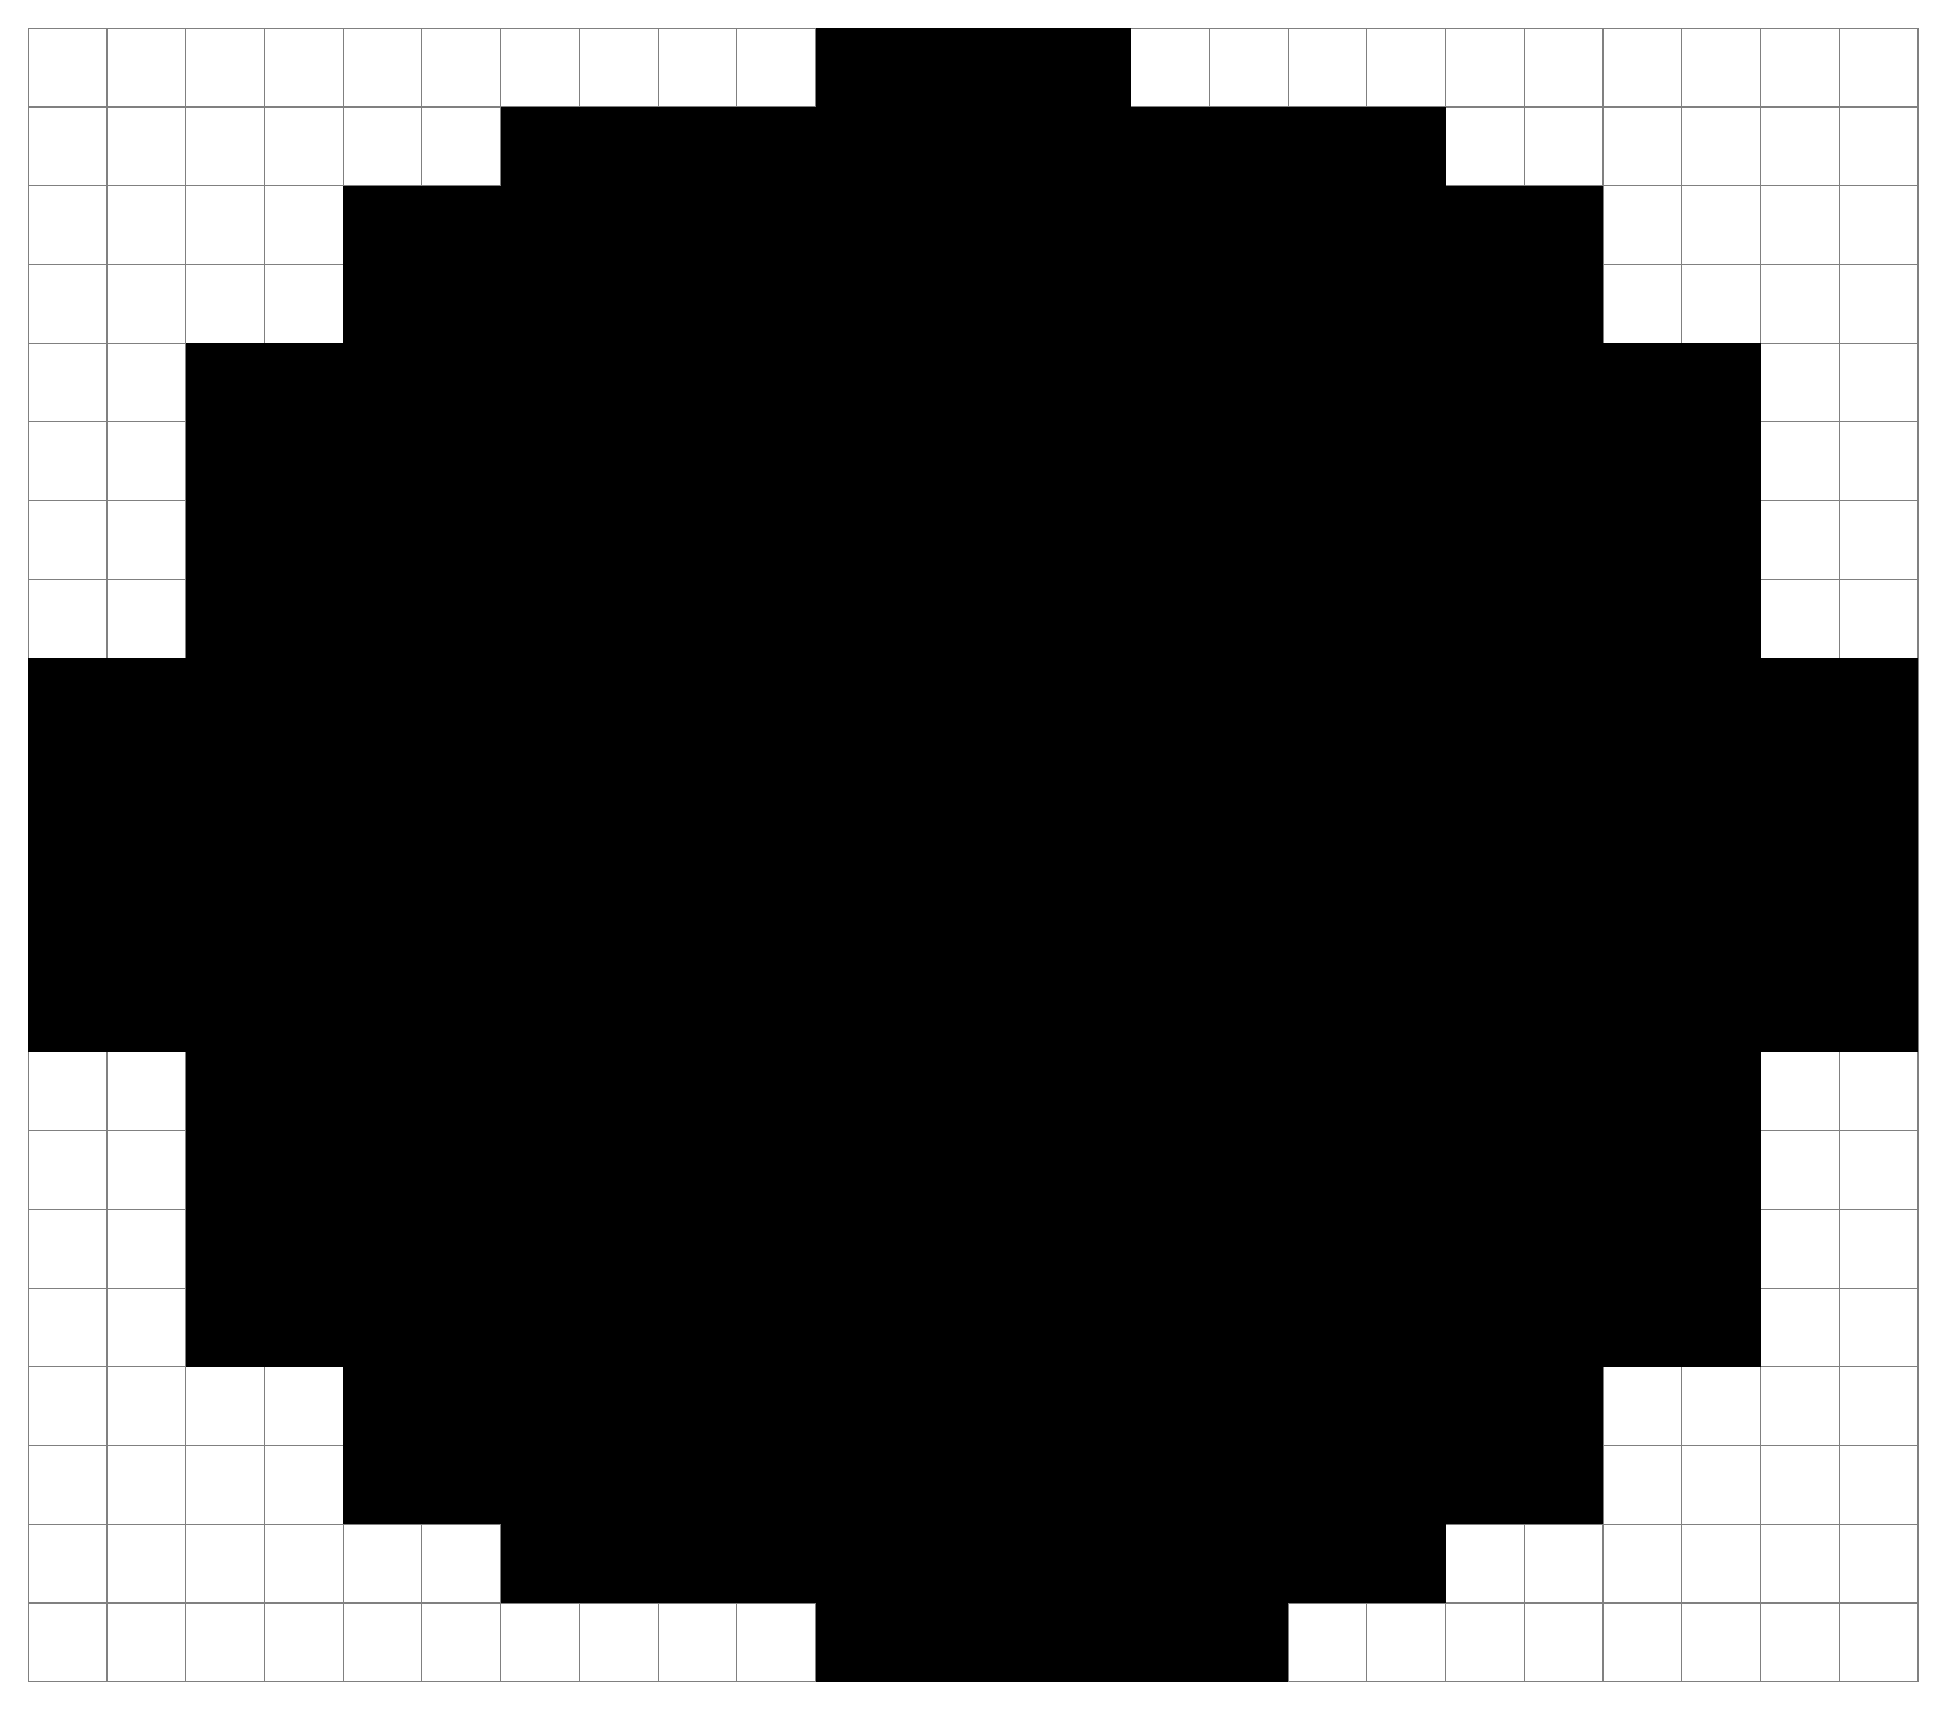
\begin{tikzpicture}

	\draw[step=1.0,gray,thin] (0,0) grid (24,21);
	\fill[\SPRITECOLOR] (10,20) rectangle ++ (1,1);
	\fill[\SPRITECOLOR] (11,20) rectangle ++ (1,1);
	\fill[\SPRITECOLOR] (12,20) rectangle ++ (1,1);
	\fill[\SPRITECOLOR] (13,20) rectangle ++ (1,1);
	\fill[\SPRITECOLOR] (6,19) rectangle ++ (1,1);
	\fill[\SPRITECOLOR] (7,19) rectangle ++ (1,1);
	\fill[\SPRITECOLOR] (8,19) rectangle ++ (1,1);
	\fill[\SPRITECOLOR] (9,19) rectangle ++ (1,1);
	\fill[\SPRITECOLOR] (10,19) rectangle ++ (1,1);
	\fill[\SPRITECOLOR] (11,19) rectangle ++ (1,1);
	\fill[\SPRITECOLOR] (12,19) rectangle ++ (1,1);
	\fill[\SPRITECOLOR] (13,19) rectangle ++ (1,1);
	\fill[\SPRITECOLOR] (14,19) rectangle ++ (1,1);
	\fill[\SPRITECOLOR] (15,19) rectangle ++ (1,1);
	\fill[\SPRITECOLOR] (16,19) rectangle ++ (1,1);
	\fill[\SPRITECOLOR] (17,19) rectangle ++ (1,1);
	\fill[\SPRITECOLOR] (4,18) rectangle ++ (1,1);
	\fill[\SPRITECOLOR] (5,18) rectangle ++ (1,1);
	\fill[\SPRITECOLOR] (6,18) rectangle ++ (1,1);
	\fill[\SPRITECOLOR] (7,18) rectangle ++ (1,1);
	\fill[\SPRITECOLOR] (8,18) rectangle ++ (1,1);
	\fill[\SPRITECOLOR] (9,18) rectangle ++ (1,1);
	\fill[\SPRITECOLOR] (10,18) rectangle ++ (1,1);
	\fill[\SPRITECOLOR] (11,18) rectangle ++ (1,1);
	\fill[\SPRITECOLOR] (12,18) rectangle ++ (1,1);
	\fill[\SPRITECOLOR] (13,18) rectangle ++ (1,1);
	\fill[\SPRITECOLOR] (14,18) rectangle ++ (1,1);
	\fill[\SPRITECOLOR] (15,18) rectangle ++ (1,1);
	\fill[\SPRITECOLOR] (16,18) rectangle ++ (1,1);
	\fill[\SPRITECOLOR] (17,18) rectangle ++ (1,1);
	\fill[\SPRITECOLOR] (18,18) rectangle ++ (1,1);
	\fill[\SPRITECOLOR] (19,18) rectangle ++ (1,1);
	\fill[\SPRITECOLOR] (4,17) rectangle ++ (1,1);
	\fill[\SPRITECOLOR] (5,17) rectangle ++ (1,1);
	\fill[\SPRITECOLOR] (6,17) rectangle ++ (1,1);
	\fill[\SPRITECOLOR] (7,17) rectangle ++ (1,1);
	\fill[\MULTICOLORTWO] (8,17) rectangle ++ (1,1);
	\fill[\MULTICOLORTWO] (9,17) rectangle ++ (1,1);
	\fill[\SPRITECOLOR] (10,17) rectangle ++ (1,1);
	\fill[\SPRITECOLOR] (11,17) rectangle ++ (1,1);
	\fill[\SPRITECOLOR] (12,17) rectangle ++ (1,1);
	\fill[\SPRITECOLOR] (13,17) rectangle ++ (1,1);
	\fill[\SPRITECOLOR] (14,17) rectangle ++ (1,1);
	\fill[\SPRITECOLOR] (15,17) rectangle ++ (1,1);
	\fill[\SPRITECOLOR] (16,17) rectangle ++ (1,1);
	\fill[\SPRITECOLOR] (17,17) rectangle ++ (1,1);
	\fill[\SPRITECOLOR] (18,17) rectangle ++ (1,1);
	\fill[\SPRITECOLOR] (19,17) rectangle ++ (1,1);
	\fill[\SPRITECOLOR] (2,16) rectangle ++ (1,1);
	\fill[\SPRITECOLOR] (3,16) rectangle ++ (1,1);
	\fill[\SPRITECOLOR] (4,16) rectangle ++ (1,1);
	\fill[\SPRITECOLOR] (5,16) rectangle ++ (1,1);
	\fill[\MULTICOLORTWO] (6,16) rectangle ++ (1,1);
	\fill[\MULTICOLORTWO] (7,16) rectangle ++ (1,1);
	\fill[\SPRITECOLOR] (8,16) rectangle ++ (1,1);
	\fill[\SPRITECOLOR] (9,16) rectangle ++ (1,1);
	\fill[\SPRITECOLOR] (10,16) rectangle ++ (1,1);
	\fill[\SPRITECOLOR] (11,16) rectangle ++ (1,1);
	\fill[\SPRITECOLOR] (12,16) rectangle ++ (1,1);
	\fill[\SPRITECOLOR] (13,16) rectangle ++ (1,1);
	\fill[\SPRITECOLOR] (14,16) rectangle ++ (1,1);
	\fill[\SPRITECOLOR] (15,16) rectangle ++ (1,1);
	\fill[\SPRITECOLOR] (16,16) rectangle ++ (1,1);
	\fill[\SPRITECOLOR] (17,16) rectangle ++ (1,1);
	\fill[\SPRITECOLOR] (18,16) rectangle ++ (1,1);
	\fill[\SPRITECOLOR] (19,16) rectangle ++ (1,1);
	\fill[\SPRITECOLOR] (20,16) rectangle ++ (1,1);
	\fill[\SPRITECOLOR] (21,16) rectangle ++ (1,1);
	\fill[\SPRITECOLOR] (2,15) rectangle ++ (1,1);
	\fill[\SPRITECOLOR] (3,15) rectangle ++ (1,1);
	\fill[\SPRITECOLOR] (4,15) rectangle ++ (1,1);
	\fill[\SPRITECOLOR] (5,15) rectangle ++ (1,1);
	\fill[\SPRITECOLOR] (6,15) rectangle ++ (1,1);
	\fill[\SPRITECOLOR] (7,15) rectangle ++ (1,1);
	\fill[\SPRITECOLOR] (8,15) rectangle ++ (1,1);
	\fill[\SPRITECOLOR] (9,15) rectangle ++ (1,1);
	\fill[\SPRITECOLOR] (10,15) rectangle ++ (1,1);
	\fill[\SPRITECOLOR] (11,15) rectangle ++ (1,1);
	\fill[\SPRITECOLOR] (12,15) rectangle ++ (1,1);
	\fill[\SPRITECOLOR] (13,15) rectangle ++ (1,1);
	\fill[\SPRITECOLOR] (14,15) rectangle ++ (1,1);
	\fill[\SPRITECOLOR] (15,15) rectangle ++ (1,1);
	\fill[\SPRITECOLOR] (16,15) rectangle ++ (1,1);
	\fill[\SPRITECOLOR] (17,15) rectangle ++ (1,1);
	\fill[\SPRITECOLOR] (18,15) rectangle ++ (1,1);
	\fill[\SPRITECOLOR] (19,15) rectangle ++ (1,1);
	\fill[\SPRITECOLOR] (20,15) rectangle ++ (1,1);
	\fill[\SPRITECOLOR] (21,15) rectangle ++ (1,1);
	\fill[\SPRITECOLOR] (2,14) rectangle ++ (1,1);
	\fill[\SPRITECOLOR] (3,14) rectangle ++ (1,1);
	\fill[\SPRITECOLOR] (4,14) rectangle ++ (1,1);
	\fill[\SPRITECOLOR] (5,14) rectangle ++ (1,1);
	\fill[\SPRITECOLOR] (6,14) rectangle ++ (1,1);
	\fill[\SPRITECOLOR] (7,14) rectangle ++ (1,1);
	\fill[\SPRITECOLOR] (8,14) rectangle ++ (1,1);
	\fill[\SPRITECOLOR] (9,14) rectangle ++ (1,1);
	\fill[\SPRITECOLOR] (10,14) rectangle ++ (1,1);
	\fill[\SPRITECOLOR] (11,14) rectangle ++ (1,1);
	\fill[\SPRITECOLOR] (12,14) rectangle ++ (1,1);
	\fill[\SPRITECOLOR] (13,14) rectangle ++ (1,1);
	\fill[\SPRITECOLOR] (14,14) rectangle ++ (1,1);
	\fill[\SPRITECOLOR] (15,14) rectangle ++ (1,1);
	\fill[\SPRITECOLOR] (16,14) rectangle ++ (1,1);
	\fill[\SPRITECOLOR] (17,14) rectangle ++ (1,1);
	\fill[\SPRITECOLOR] (18,14) rectangle ++ (1,1);
	\fill[\SPRITECOLOR] (19,14) rectangle ++ (1,1);
	\fill[\SPRITECOLOR] (20,14) rectangle ++ (1,1);
	\fill[\SPRITECOLOR] (21,14) rectangle ++ (1,1);
	\fill[\SPRITECOLOR] (2,13) rectangle ++ (1,1);
	\fill[\SPRITECOLOR] (3,13) rectangle ++ (1,1);
	\fill[\SPRITECOLOR] (4,13) rectangle ++ (1,1);
	\fill[\SPRITECOLOR] (5,13) rectangle ++ (1,1);
	\fill[\SPRITECOLOR] (6,13) rectangle ++ (1,1);
	\fill[\SPRITECOLOR] (7,13) rectangle ++ (1,1);
	\fill[\SPRITECOLOR] (8,13) rectangle ++ (1,1);
	\fill[\SPRITECOLOR] (9,13) rectangle ++ (1,1);
	\fill[\SPRITECOLOR] (10,13) rectangle ++ (1,1);
	\fill[\SPRITECOLOR] (11,13) rectangle ++ (1,1);
	\fill[\SPRITECOLOR] (12,13) rectangle ++ (1,1);
	\fill[\SPRITECOLOR] (13,13) rectangle ++ (1,1);
	\fill[\SPRITECOLOR] (14,13) rectangle ++ (1,1);
	\fill[\SPRITECOLOR] (15,13) rectangle ++ (1,1);
	\fill[\SPRITECOLOR] (16,13) rectangle ++ (1,1);
	\fill[\SPRITECOLOR] (17,13) rectangle ++ (1,1);
	\fill[\SPRITECOLOR] (18,13) rectangle ++ (1,1);
	\fill[\SPRITECOLOR] (19,13) rectangle ++ (1,1);
	\fill[\SPRITECOLOR] (20,13) rectangle ++ (1,1);
	\fill[\SPRITECOLOR] (21,13) rectangle ++ (1,1);
	\fill[\SPRITECOLOR] (0,12) rectangle ++ (1,1);
	\fill[\SPRITECOLOR] (1,12) rectangle ++ (1,1);
	\fill[\SPRITECOLOR] (2,12) rectangle ++ (1,1);
	\fill[\SPRITECOLOR] (3,12) rectangle ++ (1,1);
	\fill[\SPRITECOLOR] (4,12) rectangle ++ (1,1);
	\fill[\SPRITECOLOR] (5,12) rectangle ++ (1,1);
	\fill[\SPRITECOLOR] (6,12) rectangle ++ (1,1);
	\fill[\SPRITECOLOR] (7,12) rectangle ++ (1,1);
	\fill[\MULTICOLORTWO] (8,12) rectangle ++ (1,1);
	\fill[\MULTICOLORTWO] (9,12) rectangle ++ (1,1);
	\fill[\MULTICOLORTWO] (10,12) rectangle ++ (1,1);
	\fill[\MULTICOLORTWO] (11,12) rectangle ++ (1,1);
	\fill[\MULTICOLORTWO] (12,12) rectangle ++ (1,1);
	\fill[\MULTICOLORTWO] (13,12) rectangle ++ (1,1);
	\fill[\MULTICOLORTWO] (14,12) rectangle ++ (1,1);
	\fill[\MULTICOLORTWO] (15,12) rectangle ++ (1,1);
	\fill[\MULTICOLORTWO] (16,12) rectangle ++ (1,1);
	\fill[\MULTICOLORTWO] (17,12) rectangle ++ (1,1);
	\fill[\SPRITECOLOR] (18,12) rectangle ++ (1,1);
	\fill[\SPRITECOLOR] (19,12) rectangle ++ (1,1);
	\fill[\SPRITECOLOR] (20,12) rectangle ++ (1,1);
	\fill[\SPRITECOLOR] (21,12) rectangle ++ (1,1);
	\fill[\SPRITECOLOR] (22,12) rectangle ++ (1,1);
	\fill[\SPRITECOLOR] (23,12) rectangle ++ (1,1);
	\fill[\SPRITECOLOR] (0,11) rectangle ++ (1,1);
	\fill[\SPRITECOLOR] (1,11) rectangle ++ (1,1);
	\fill[\SPRITECOLOR] (2,11) rectangle ++ (1,1);
	\fill[\SPRITECOLOR] (3,11) rectangle ++ (1,1);
	\fill[\MULTICOLORTWO] (4,11) rectangle ++ (1,1);
	\fill[\MULTICOLORTWO] (5,11) rectangle ++ (1,1);
	\fill[\MULTICOLORTWO] (6,11) rectangle ++ (1,1);
	\fill[\MULTICOLORTWO] (7,11) rectangle ++ (1,1);
	\fill[\MULTICOLORTWO] (8,11) rectangle ++ (1,1);
	\fill[\MULTICOLORTWO] (9,11) rectangle ++ (1,1);
	\fill[\MULTICOLORONE] (10,11) rectangle ++ (1,1);
	\fill[\MULTICOLORONE] (11,11) rectangle ++ (1,1);
	\fill[\MULTICOLORONE] (12,11) rectangle ++ (1,1);
	\fill[\MULTICOLORONE] (13,11) rectangle ++ (1,1);
	\fill[\MULTICOLORONE] (14,11) rectangle ++ (1,1);
	\fill[\MULTICOLORONE] (15,11) rectangle ++ (1,1);
	\fill[\MULTICOLORTWO] (16,11) rectangle ++ (1,1);
	\fill[\MULTICOLORTWO] (17,11) rectangle ++ (1,1);
	\fill[\MULTICOLORTWO] (18,11) rectangle ++ (1,1);
	\fill[\MULTICOLORTWO] (19,11) rectangle ++ (1,1);
	\fill[\SPRITECOLOR] (20,11) rectangle ++ (1,1);
	\fill[\SPRITECOLOR] (21,11) rectangle ++ (1,1);
	\fill[\SPRITECOLOR] (22,11) rectangle ++ (1,1);
	\fill[\SPRITECOLOR] (23,11) rectangle ++ (1,1);
	\fill[\SPRITECOLOR] (0,10) rectangle ++ (1,1);
	\fill[\SPRITECOLOR] (1,10) rectangle ++ (1,1);
	\fill[\SPRITECOLOR] (2,10) rectangle ++ (1,1);
	\fill[\SPRITECOLOR] (3,10) rectangle ++ (1,1);
	\fill[\MULTICOLORTWO] (4,10) rectangle ++ (1,1);
	\fill[\MULTICOLORTWO] (5,10) rectangle ++ (1,1);
	\fill[\MULTICOLORTWO] (6,10) rectangle ++ (1,1);
	\fill[\MULTICOLORTWO] (7,10) rectangle ++ (1,1);
	\fill[\MULTICOLORTWO] (8,10) rectangle ++ (1,1);
	\fill[\MULTICOLORTWO] (9,10) rectangle ++ (1,1);
	\fill[\MULTICOLORONE] (10,10) rectangle ++ (1,1);
	\fill[\MULTICOLORONE] (11,10) rectangle ++ (1,1);
	\fill[\MULTICOLORONE] (12,10) rectangle ++ (1,1);
	\fill[\MULTICOLORONE] (13,10) rectangle ++ (1,1);
	\fill[\MULTICOLORONE] (14,10) rectangle ++ (1,1);
	\fill[\MULTICOLORONE] (15,10) rectangle ++ (1,1);
	\fill[\MULTICOLORTWO] (16,10) rectangle ++ (1,1);
	\fill[\MULTICOLORTWO] (17,10) rectangle ++ (1,1);
	\fill[\MULTICOLORTWO] (18,10) rectangle ++ (1,1);
	\fill[\MULTICOLORTWO] (19,10) rectangle ++ (1,1);
	\fill[\MULTICOLORTWO] (20,10) rectangle ++ (1,1);
	\fill[\MULTICOLORTWO] (21,10) rectangle ++ (1,1);
	\fill[\SPRITECOLOR] (22,10) rectangle ++ (1,1);
	\fill[\SPRITECOLOR] (23,10) rectangle ++ (1,1);
	\fill[\SPRITECOLOR] (0,9) rectangle ++ (1,1);
	\fill[\SPRITECOLOR] (1,9) rectangle ++ (1,1);
	\fill[\SPRITECOLOR] (2,9) rectangle ++ (1,1);
	\fill[\SPRITECOLOR] (3,9) rectangle ++ (1,1);
	\fill[\SPRITECOLOR] (4,9) rectangle ++ (1,1);
	\fill[\SPRITECOLOR] (5,9) rectangle ++ (1,1);
	\fill[\MULTICOLORTWO] (6,9) rectangle ++ (1,1);
	\fill[\MULTICOLORTWO] (7,9) rectangle ++ (1,1);
	\fill[\MULTICOLORTWO] (8,9) rectangle ++ (1,1);
	\fill[\MULTICOLORTWO] (9,9) rectangle ++ (1,1);
	\fill[\MULTICOLORONE] (10,9) rectangle ++ (1,1);
	\fill[\MULTICOLORONE] (11,9) rectangle ++ (1,1);
	\fill[\MULTICOLORONE] (12,9) rectangle ++ (1,1);
	\fill[\MULTICOLORONE] (13,9) rectangle ++ (1,1);
	\fill[\MULTICOLORONE] (14,9) rectangle ++ (1,1);
	\fill[\MULTICOLORONE] (15,9) rectangle ++ (1,1);
	\fill[\MULTICOLORTWO] (16,9) rectangle ++ (1,1);
	\fill[\MULTICOLORTWO] (17,9) rectangle ++ (1,1);
	\fill[\MULTICOLORTWO] (18,9) rectangle ++ (1,1);
	\fill[\MULTICOLORTWO] (19,9) rectangle ++ (1,1);
	\fill[\MULTICOLORTWO] (20,9) rectangle ++ (1,1);
	\fill[\MULTICOLORTWO] (21,9) rectangle ++ (1,1);
	\fill[\SPRITECOLOR] (22,9) rectangle ++ (1,1);
	\fill[\SPRITECOLOR] (23,9) rectangle ++ (1,1);
	\fill[\SPRITECOLOR] (0,8) rectangle ++ (1,1);
	\fill[\SPRITECOLOR] (1,8) rectangle ++ (1,1);
	\fill[\SPRITECOLOR] (2,8) rectangle ++ (1,1);
	\fill[\SPRITECOLOR] (3,8) rectangle ++ (1,1);
	\fill[\SPRITECOLOR] (4,8) rectangle ++ (1,1);
	\fill[\SPRITECOLOR] (5,8) rectangle ++ (1,1);
	\fill[\SPRITECOLOR] (6,8) rectangle ++ (1,1);
	\fill[\SPRITECOLOR] (7,8) rectangle ++ (1,1);
	\fill[\MULTICOLORTWO] (8,8) rectangle ++ (1,1);
	\fill[\MULTICOLORTWO] (9,8) rectangle ++ (1,1);
	\fill[\MULTICOLORTWO] (10,8) rectangle ++ (1,1);
	\fill[\MULTICOLORTWO] (11,8) rectangle ++ (1,1);
	\fill[\MULTICOLORTWO] (12,8) rectangle ++ (1,1);
	\fill[\MULTICOLORTWO] (13,8) rectangle ++ (1,1);
	\fill[\MULTICOLORTWO] (14,8) rectangle ++ (1,1);
	\fill[\MULTICOLORTWO] (15,8) rectangle ++ (1,1);
	\fill[\MULTICOLORTWO] (16,8) rectangle ++ (1,1);
	\fill[\MULTICOLORTWO] (17,8) rectangle ++ (1,1);
	\fill[\SPRITECOLOR] (18,8) rectangle ++ (1,1);
	\fill[\SPRITECOLOR] (19,8) rectangle ++ (1,1);
	\fill[\SPRITECOLOR] (20,8) rectangle ++ (1,1);
	\fill[\SPRITECOLOR] (21,8) rectangle ++ (1,1);
	\fill[\SPRITECOLOR] (22,8) rectangle ++ (1,1);
	\fill[\SPRITECOLOR] (23,8) rectangle ++ (1,1);
	\fill[\SPRITECOLOR] (2,7) rectangle ++ (1,1);
	\fill[\SPRITECOLOR] (3,7) rectangle ++ (1,1);
	\fill[\SPRITECOLOR] (4,7) rectangle ++ (1,1);
	\fill[\SPRITECOLOR] (5,7) rectangle ++ (1,1);
	\fill[\SPRITECOLOR] (6,7) rectangle ++ (1,1);
	\fill[\SPRITECOLOR] (7,7) rectangle ++ (1,1);
	\fill[\SPRITECOLOR] (8,7) rectangle ++ (1,1);
	\fill[\SPRITECOLOR] (9,7) rectangle ++ (1,1);
	\fill[\SPRITECOLOR] (10,7) rectangle ++ (1,1);
	\fill[\SPRITECOLOR] (11,7) rectangle ++ (1,1);
	\fill[\SPRITECOLOR] (12,7) rectangle ++ (1,1);
	\fill[\SPRITECOLOR] (13,7) rectangle ++ (1,1);
	\fill[\SPRITECOLOR] (14,7) rectangle ++ (1,1);
	\fill[\SPRITECOLOR] (15,7) rectangle ++ (1,1);
	\fill[\SPRITECOLOR] (16,7) rectangle ++ (1,1);
	\fill[\SPRITECOLOR] (17,7) rectangle ++ (1,1);
	\fill[\SPRITECOLOR] (18,7) rectangle ++ (1,1);
	\fill[\SPRITECOLOR] (19,7) rectangle ++ (1,1);
	\fill[\SPRITECOLOR] (20,7) rectangle ++ (1,1);
	\fill[\SPRITECOLOR] (21,7) rectangle ++ (1,1);
	\fill[\SPRITECOLOR] (2,6) rectangle ++ (1,1);
	\fill[\SPRITECOLOR] (3,6) rectangle ++ (1,1);
	\fill[\SPRITECOLOR] (4,6) rectangle ++ (1,1);
	\fill[\SPRITECOLOR] (5,6) rectangle ++ (1,1);
	\fill[\SPRITECOLOR] (6,6) rectangle ++ (1,1);
	\fill[\SPRITECOLOR] (7,6) rectangle ++ (1,1);
	\fill[\SPRITECOLOR] (8,6) rectangle ++ (1,1);
	\fill[\SPRITECOLOR] (9,6) rectangle ++ (1,1);
	\fill[\SPRITECOLOR] (10,6) rectangle ++ (1,1);
	\fill[\SPRITECOLOR] (11,6) rectangle ++ (1,1);
	\fill[\SPRITECOLOR] (12,6) rectangle ++ (1,1);
	\fill[\SPRITECOLOR] (13,6) rectangle ++ (1,1);
	\fill[\SPRITECOLOR] (14,6) rectangle ++ (1,1);
	\fill[\SPRITECOLOR] (15,6) rectangle ++ (1,1);
	\fill[\SPRITECOLOR] (16,6) rectangle ++ (1,1);
	\fill[\SPRITECOLOR] (17,6) rectangle ++ (1,1);
	\fill[\SPRITECOLOR] (18,6) rectangle ++ (1,1);
	\fill[\SPRITECOLOR] (19,6) rectangle ++ (1,1);
	\fill[\SPRITECOLOR] (20,6) rectangle ++ (1,1);
	\fill[\SPRITECOLOR] (21,6) rectangle ++ (1,1);
	\fill[\SPRITECOLOR] (2,5) rectangle ++ (1,1);
	\fill[\SPRITECOLOR] (3,5) rectangle ++ (1,1);
	\fill[\SPRITECOLOR] (4,5) rectangle ++ (1,1);
	\fill[\SPRITECOLOR] (5,5) rectangle ++ (1,1);
	\fill[\SPRITECOLOR] (6,5) rectangle ++ (1,1);
	\fill[\SPRITECOLOR] (7,5) rectangle ++ (1,1);
	\fill[\SPRITECOLOR] (8,5) rectangle ++ (1,1);
	\fill[\SPRITECOLOR] (9,5) rectangle ++ (1,1);
	\fill[\SPRITECOLOR] (10,5) rectangle ++ (1,1);
	\fill[\SPRITECOLOR] (11,5) rectangle ++ (1,1);
	\fill[\SPRITECOLOR] (12,5) rectangle ++ (1,1);
	\fill[\SPRITECOLOR] (13,5) rectangle ++ (1,1);
	\fill[\SPRITECOLOR] (14,5) rectangle ++ (1,1);
	\fill[\SPRITECOLOR] (15,5) rectangle ++ (1,1);
	\fill[\SPRITECOLOR] (16,5) rectangle ++ (1,1);
	\fill[\SPRITECOLOR] (17,5) rectangle ++ (1,1);
	\fill[\SPRITECOLOR] (18,5) rectangle ++ (1,1);
	\fill[\SPRITECOLOR] (19,5) rectangle ++ (1,1);
	\fill[\SPRITECOLOR] (20,5) rectangle ++ (1,1);
	\fill[\SPRITECOLOR] (21,5) rectangle ++ (1,1);
	\fill[\SPRITECOLOR] (2,4) rectangle ++ (1,1);
	\fill[\SPRITECOLOR] (3,4) rectangle ++ (1,1);
	\fill[\SPRITECOLOR] (4,4) rectangle ++ (1,1);
	\fill[\SPRITECOLOR] (5,4) rectangle ++ (1,1);
	\fill[\SPRITECOLOR] (6,4) rectangle ++ (1,1);
	\fill[\SPRITECOLOR] (7,4) rectangle ++ (1,1);
	\fill[\SPRITECOLOR] (8,4) rectangle ++ (1,1);
	\fill[\SPRITECOLOR] (9,4) rectangle ++ (1,1);
	\fill[\SPRITECOLOR] (10,4) rectangle ++ (1,1);
	\fill[\SPRITECOLOR] (11,4) rectangle ++ (1,1);
	\fill[\SPRITECOLOR] (12,4) rectangle ++ (1,1);
	\fill[\SPRITECOLOR] (13,4) rectangle ++ (1,1);
	\fill[\SPRITECOLOR] (14,4) rectangle ++ (1,1);
	\fill[\SPRITECOLOR] (15,4) rectangle ++ (1,1);
	\fill[\SPRITECOLOR] (16,4) rectangle ++ (1,1);
	\fill[\SPRITECOLOR] (17,4) rectangle ++ (1,1);
	\fill[\SPRITECOLOR] (18,4) rectangle ++ (1,1);
	\fill[\SPRITECOLOR] (19,4) rectangle ++ (1,1);
	\fill[\SPRITECOLOR] (20,4) rectangle ++ (1,1);
	\fill[\SPRITECOLOR] (21,4) rectangle ++ (1,1);
	\fill[\SPRITECOLOR] (4,3) rectangle ++ (1,1);
	\fill[\SPRITECOLOR] (5,3) rectangle ++ (1,1);
	\fill[\SPRITECOLOR] (6,3) rectangle ++ (1,1);
	\fill[\SPRITECOLOR] (7,3) rectangle ++ (1,1);
	\fill[\SPRITECOLOR] (8,3) rectangle ++ (1,1);
	\fill[\SPRITECOLOR] (9,3) rectangle ++ (1,1);
	\fill[\SPRITECOLOR] (10,3) rectangle ++ (1,1);
	\fill[\SPRITECOLOR] (11,3) rectangle ++ (1,1);
	\fill[\SPRITECOLOR] (12,3) rectangle ++ (1,1);
	\fill[\SPRITECOLOR] (13,3) rectangle ++ (1,1);
	\fill[\SPRITECOLOR] (14,3) rectangle ++ (1,1);
	\fill[\SPRITECOLOR] (15,3) rectangle ++ (1,1);
	\fill[\SPRITECOLOR] (16,3) rectangle ++ (1,1);
	\fill[\SPRITECOLOR] (17,3) rectangle ++ (1,1);
	\fill[\SPRITECOLOR] (18,3) rectangle ++ (1,1);
	\fill[\SPRITECOLOR] (19,3) rectangle ++ (1,1);
	\fill[\SPRITECOLOR] (4,2) rectangle ++ (1,1);
	\fill[\SPRITECOLOR] (5,2) rectangle ++ (1,1);
	\fill[\SPRITECOLOR] (6,2) rectangle ++ (1,1);
	\fill[\SPRITECOLOR] (7,2) rectangle ++ (1,1);
	\fill[\SPRITECOLOR] (8,2) rectangle ++ (1,1);
	\fill[\SPRITECOLOR] (9,2) rectangle ++ (1,1);
	\fill[\SPRITECOLOR] (10,2) rectangle ++ (1,1);
	\fill[\SPRITECOLOR] (11,2) rectangle ++ (1,1);
	\fill[\SPRITECOLOR] (12,2) rectangle ++ (1,1);
	\fill[\SPRITECOLOR] (13,2) rectangle ++ (1,1);
	\fill[\SPRITECOLOR] (14,2) rectangle ++ (1,1);
	\fill[\SPRITECOLOR] (15,2) rectangle ++ (1,1);
	\fill[\SPRITECOLOR] (16,2) rectangle ++ (1,1);
	\fill[\SPRITECOLOR] (17,2) rectangle ++ (1,1);
	\fill[\SPRITECOLOR] (18,2) rectangle ++ (1,1);
	\fill[\SPRITECOLOR] (19,2) rectangle ++ (1,1);
	\fill[\SPRITECOLOR] (6,1) rectangle ++ (1,1);
	\fill[\SPRITECOLOR] (7,1) rectangle ++ (1,1);
	\fill[\SPRITECOLOR] (8,1) rectangle ++ (1,1);
	\fill[\SPRITECOLOR] (9,1) rectangle ++ (1,1);
	\fill[\SPRITECOLOR] (10,1) rectangle ++ (1,1);
	\fill[\SPRITECOLOR] (11,1) rectangle ++ (1,1);
	\fill[\SPRITECOLOR] (12,1) rectangle ++ (1,1);
	\fill[\SPRITECOLOR] (13,1) rectangle ++ (1,1);
	\fill[\SPRITECOLOR] (14,1) rectangle ++ (1,1);
	\fill[\SPRITECOLOR] (15,1) rectangle ++ (1,1);
	\fill[\SPRITECOLOR] (16,1) rectangle ++ (1,1);
	\fill[\SPRITECOLOR] (17,1) rectangle ++ (1,1);
	\fill[\SPRITECOLOR] (10,0) rectangle ++ (1,1);
	\fill[\SPRITECOLOR] (11,0) rectangle ++ (1,1);
	\fill[\SPRITECOLOR] (12,0) rectangle ++ (1,1);
	\fill[\SPRITECOLOR] (13,0) rectangle ++ (1,1);
	\fill[\SPRITECOLOR] (14,0) rectangle ++ (1,1);
	\fill[\SPRITECOLOR] (15,0) rectangle ++ (1,1);

      \end{tikzpicture}
    \end{adjustbox}
  }\caption{BONUS\_IBALL2}
\end{figure}

	\end{subfigure}
} &
\makecell[l]{
	\begin{subfigure}{0.3\textwidth}
    \def\MULTICOLORONE{red}
    \def\MULTICOLORTWO{white}
    \def\SPRITECOLOR{lightblue}
		
\begin{figure}[H]
  {
    \setlength{\tabcolsep}{3.0pt}
    \setlength\cmidrulewidth{\heavyrulewidth} % Make cmidrule = 
    \begin{adjustbox}{width=3cm,center}
      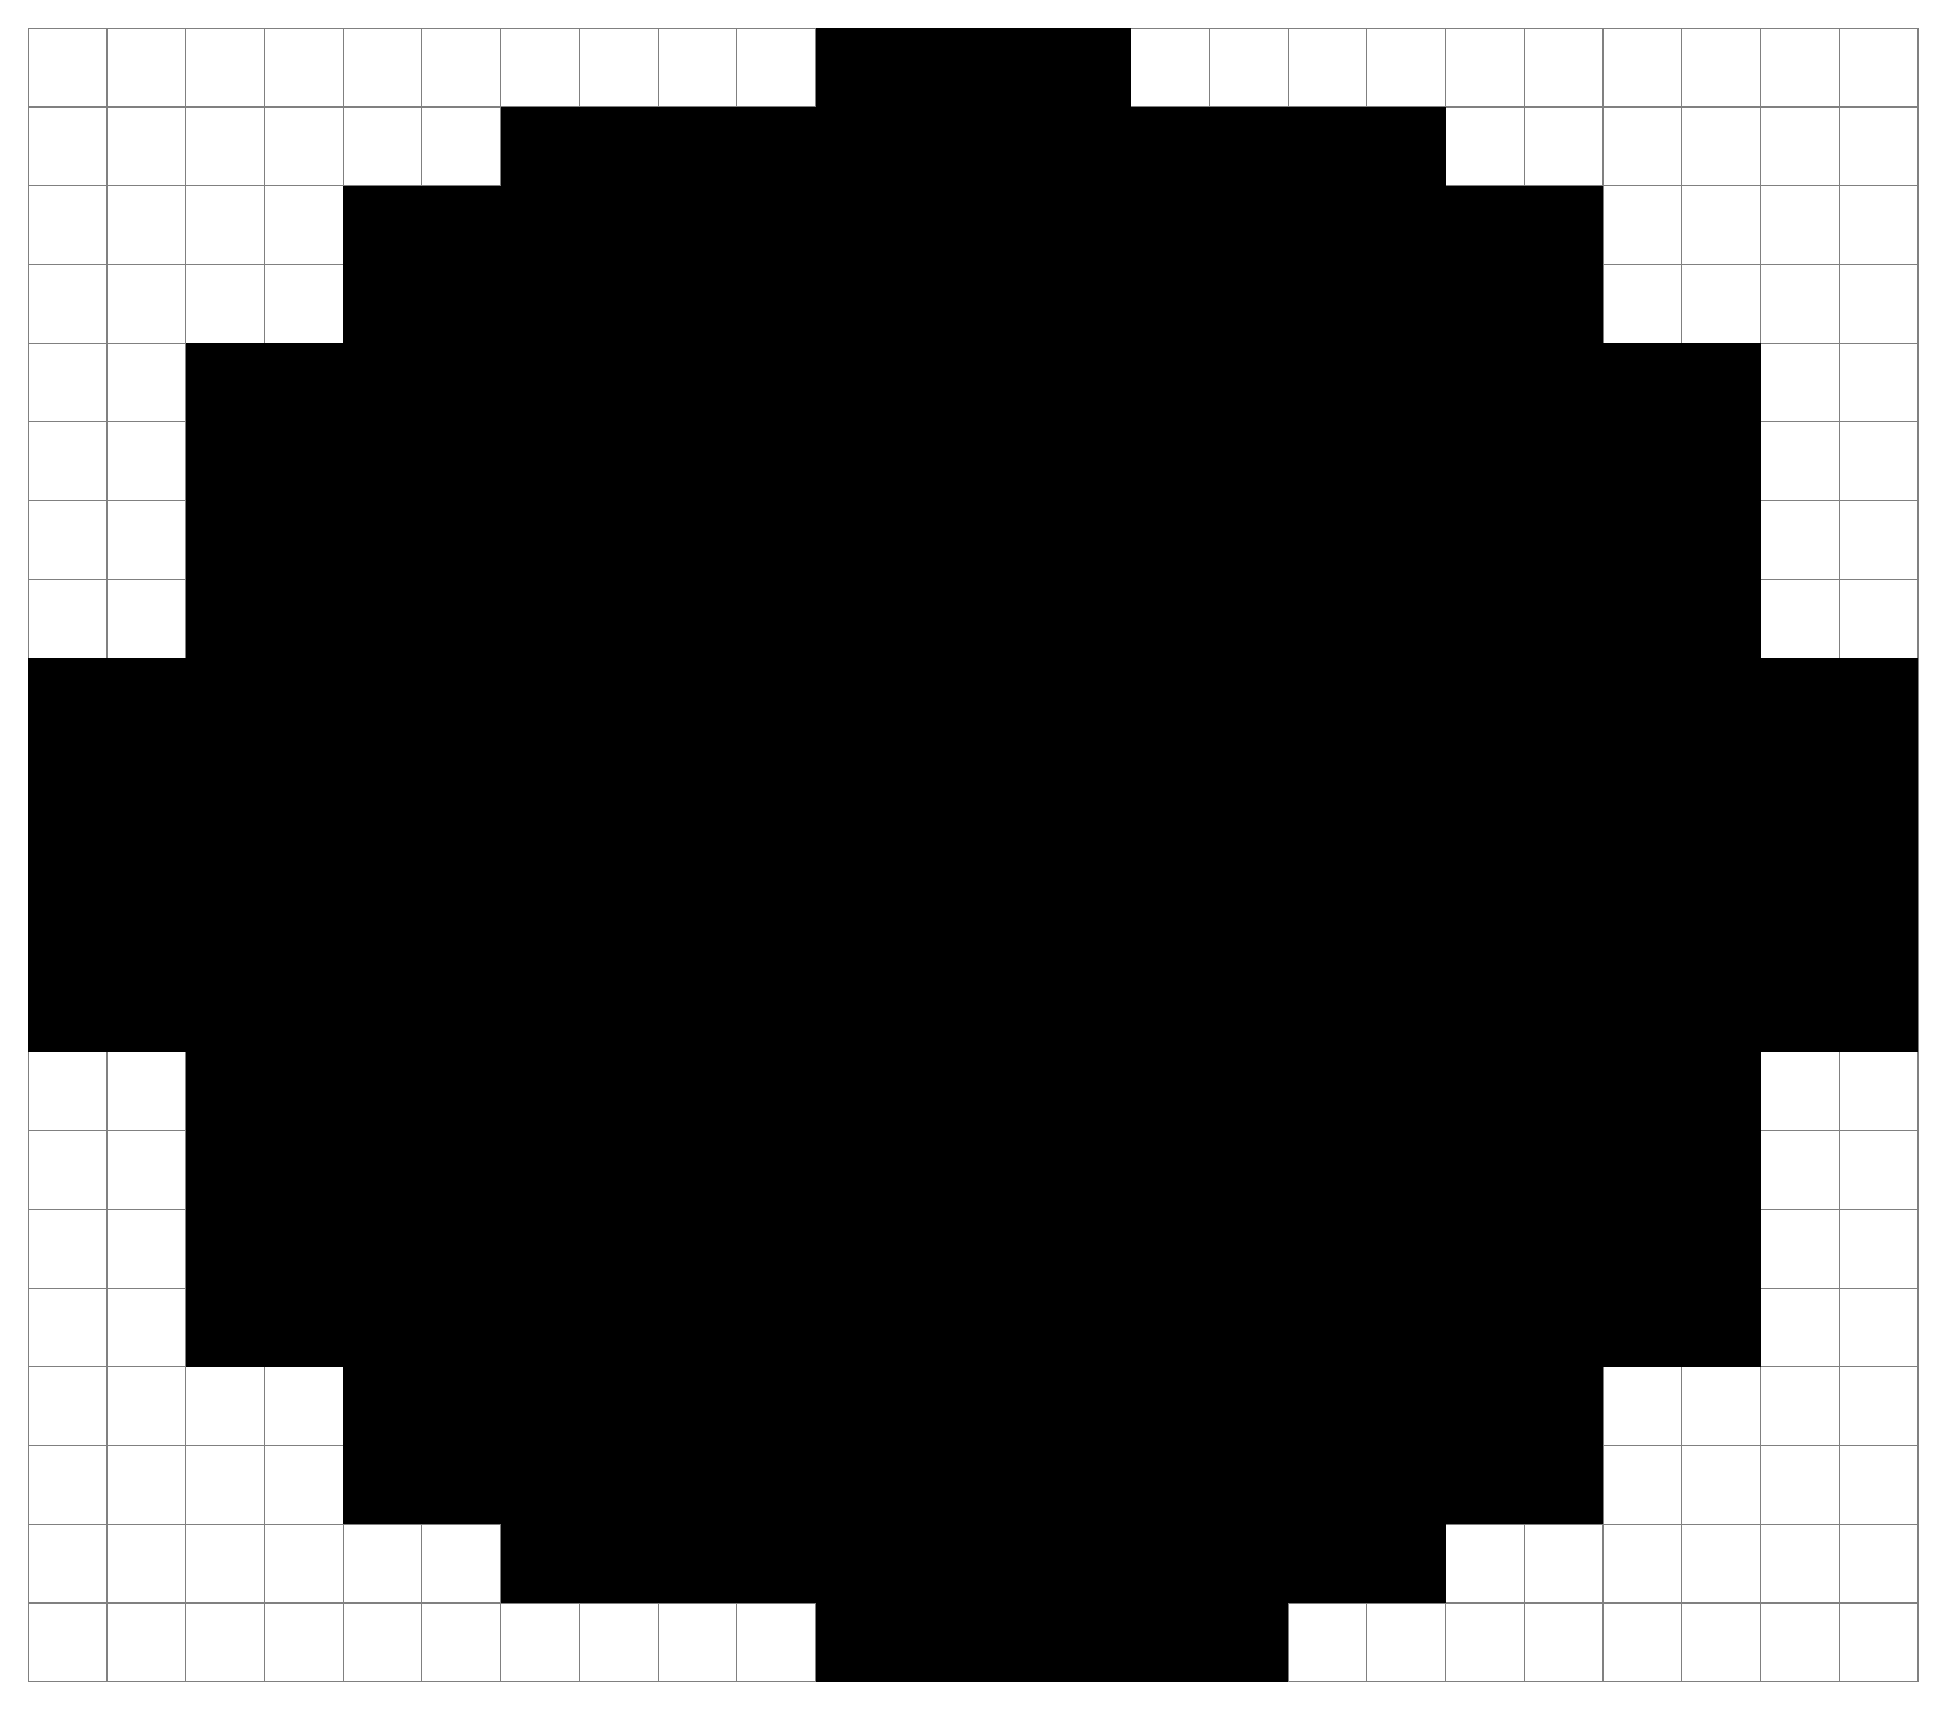
\begin{tikzpicture}

	\draw[step=1.0,gray,thin] (0,0) grid (24,21);
	\fill[\SPRITECOLOR] (10,20) rectangle ++ (1,1);
	\fill[\SPRITECOLOR] (11,20) rectangle ++ (1,1);
	\fill[\SPRITECOLOR] (12,20) rectangle ++ (1,1);
	\fill[\SPRITECOLOR] (13,20) rectangle ++ (1,1);
	\fill[\SPRITECOLOR] (6,19) rectangle ++ (1,1);
	\fill[\SPRITECOLOR] (7,19) rectangle ++ (1,1);
	\fill[\SPRITECOLOR] (8,19) rectangle ++ (1,1);
	\fill[\SPRITECOLOR] (9,19) rectangle ++ (1,1);
	\fill[\SPRITECOLOR] (10,19) rectangle ++ (1,1);
	\fill[\SPRITECOLOR] (11,19) rectangle ++ (1,1);
	\fill[\SPRITECOLOR] (12,19) rectangle ++ (1,1);
	\fill[\SPRITECOLOR] (13,19) rectangle ++ (1,1);
	\fill[\SPRITECOLOR] (14,19) rectangle ++ (1,1);
	\fill[\SPRITECOLOR] (15,19) rectangle ++ (1,1);
	\fill[\SPRITECOLOR] (16,19) rectangle ++ (1,1);
	\fill[\SPRITECOLOR] (17,19) rectangle ++ (1,1);
	\fill[\SPRITECOLOR] (4,18) rectangle ++ (1,1);
	\fill[\SPRITECOLOR] (5,18) rectangle ++ (1,1);
	\fill[\SPRITECOLOR] (6,18) rectangle ++ (1,1);
	\fill[\SPRITECOLOR] (7,18) rectangle ++ (1,1);
	\fill[\SPRITECOLOR] (8,18) rectangle ++ (1,1);
	\fill[\SPRITECOLOR] (9,18) rectangle ++ (1,1);
	\fill[\SPRITECOLOR] (10,18) rectangle ++ (1,1);
	\fill[\SPRITECOLOR] (11,18) rectangle ++ (1,1);
	\fill[\SPRITECOLOR] (12,18) rectangle ++ (1,1);
	\fill[\SPRITECOLOR] (13,18) rectangle ++ (1,1);
	\fill[\SPRITECOLOR] (14,18) rectangle ++ (1,1);
	\fill[\SPRITECOLOR] (15,18) rectangle ++ (1,1);
	\fill[\SPRITECOLOR] (16,18) rectangle ++ (1,1);
	\fill[\SPRITECOLOR] (17,18) rectangle ++ (1,1);
	\fill[\SPRITECOLOR] (18,18) rectangle ++ (1,1);
	\fill[\SPRITECOLOR] (19,18) rectangle ++ (1,1);
	\fill[\SPRITECOLOR] (4,17) rectangle ++ (1,1);
	\fill[\SPRITECOLOR] (5,17) rectangle ++ (1,1);
	\fill[\SPRITECOLOR] (6,17) rectangle ++ (1,1);
	\fill[\SPRITECOLOR] (7,17) rectangle ++ (1,1);
	\fill[\MULTICOLORTWO] (8,17) rectangle ++ (1,1);
	\fill[\MULTICOLORTWO] (9,17) rectangle ++ (1,1);
	\fill[\SPRITECOLOR] (10,17) rectangle ++ (1,1);
	\fill[\SPRITECOLOR] (11,17) rectangle ++ (1,1);
	\fill[\SPRITECOLOR] (12,17) rectangle ++ (1,1);
	\fill[\SPRITECOLOR] (13,17) rectangle ++ (1,1);
	\fill[\SPRITECOLOR] (14,17) rectangle ++ (1,1);
	\fill[\SPRITECOLOR] (15,17) rectangle ++ (1,1);
	\fill[\SPRITECOLOR] (16,17) rectangle ++ (1,1);
	\fill[\SPRITECOLOR] (17,17) rectangle ++ (1,1);
	\fill[\SPRITECOLOR] (18,17) rectangle ++ (1,1);
	\fill[\SPRITECOLOR] (19,17) rectangle ++ (1,1);
	\fill[\SPRITECOLOR] (2,16) rectangle ++ (1,1);
	\fill[\SPRITECOLOR] (3,16) rectangle ++ (1,1);
	\fill[\SPRITECOLOR] (4,16) rectangle ++ (1,1);
	\fill[\SPRITECOLOR] (5,16) rectangle ++ (1,1);
	\fill[\MULTICOLORTWO] (6,16) rectangle ++ (1,1);
	\fill[\MULTICOLORTWO] (7,16) rectangle ++ (1,1);
	\fill[\SPRITECOLOR] (8,16) rectangle ++ (1,1);
	\fill[\SPRITECOLOR] (9,16) rectangle ++ (1,1);
	\fill[\SPRITECOLOR] (10,16) rectangle ++ (1,1);
	\fill[\SPRITECOLOR] (11,16) rectangle ++ (1,1);
	\fill[\SPRITECOLOR] (12,16) rectangle ++ (1,1);
	\fill[\SPRITECOLOR] (13,16) rectangle ++ (1,1);
	\fill[\SPRITECOLOR] (14,16) rectangle ++ (1,1);
	\fill[\SPRITECOLOR] (15,16) rectangle ++ (1,1);
	\fill[\SPRITECOLOR] (16,16) rectangle ++ (1,1);
	\fill[\SPRITECOLOR] (17,16) rectangle ++ (1,1);
	\fill[\SPRITECOLOR] (18,16) rectangle ++ (1,1);
	\fill[\SPRITECOLOR] (19,16) rectangle ++ (1,1);
	\fill[\SPRITECOLOR] (20,16) rectangle ++ (1,1);
	\fill[\SPRITECOLOR] (21,16) rectangle ++ (1,1);
	\fill[\SPRITECOLOR] (2,15) rectangle ++ (1,1);
	\fill[\SPRITECOLOR] (3,15) rectangle ++ (1,1);
	\fill[\SPRITECOLOR] (4,15) rectangle ++ (1,1);
	\fill[\SPRITECOLOR] (5,15) rectangle ++ (1,1);
	\fill[\SPRITECOLOR] (6,15) rectangle ++ (1,1);
	\fill[\SPRITECOLOR] (7,15) rectangle ++ (1,1);
	\fill[\SPRITECOLOR] (8,15) rectangle ++ (1,1);
	\fill[\SPRITECOLOR] (9,15) rectangle ++ (1,1);
	\fill[\SPRITECOLOR] (10,15) rectangle ++ (1,1);
	\fill[\SPRITECOLOR] (11,15) rectangle ++ (1,1);
	\fill[\SPRITECOLOR] (12,15) rectangle ++ (1,1);
	\fill[\SPRITECOLOR] (13,15) rectangle ++ (1,1);
	\fill[\SPRITECOLOR] (14,15) rectangle ++ (1,1);
	\fill[\SPRITECOLOR] (15,15) rectangle ++ (1,1);
	\fill[\SPRITECOLOR] (16,15) rectangle ++ (1,1);
	\fill[\SPRITECOLOR] (17,15) rectangle ++ (1,1);
	\fill[\SPRITECOLOR] (18,15) rectangle ++ (1,1);
	\fill[\SPRITECOLOR] (19,15) rectangle ++ (1,1);
	\fill[\SPRITECOLOR] (20,15) rectangle ++ (1,1);
	\fill[\SPRITECOLOR] (21,15) rectangle ++ (1,1);
	\fill[\SPRITECOLOR] (2,14) rectangle ++ (1,1);
	\fill[\SPRITECOLOR] (3,14) rectangle ++ (1,1);
	\fill[\SPRITECOLOR] (4,14) rectangle ++ (1,1);
	\fill[\SPRITECOLOR] (5,14) rectangle ++ (1,1);
	\fill[\SPRITECOLOR] (6,14) rectangle ++ (1,1);
	\fill[\SPRITECOLOR] (7,14) rectangle ++ (1,1);
	\fill[\SPRITECOLOR] (8,14) rectangle ++ (1,1);
	\fill[\SPRITECOLOR] (9,14) rectangle ++ (1,1);
	\fill[\SPRITECOLOR] (10,14) rectangle ++ (1,1);
	\fill[\SPRITECOLOR] (11,14) rectangle ++ (1,1);
	\fill[\SPRITECOLOR] (12,14) rectangle ++ (1,1);
	\fill[\SPRITECOLOR] (13,14) rectangle ++ (1,1);
	\fill[\SPRITECOLOR] (14,14) rectangle ++ (1,1);
	\fill[\SPRITECOLOR] (15,14) rectangle ++ (1,1);
	\fill[\SPRITECOLOR] (16,14) rectangle ++ (1,1);
	\fill[\SPRITECOLOR] (17,14) rectangle ++ (1,1);
	\fill[\SPRITECOLOR] (18,14) rectangle ++ (1,1);
	\fill[\SPRITECOLOR] (19,14) rectangle ++ (1,1);
	\fill[\SPRITECOLOR] (20,14) rectangle ++ (1,1);
	\fill[\SPRITECOLOR] (21,14) rectangle ++ (1,1);
	\fill[\SPRITECOLOR] (2,13) rectangle ++ (1,1);
	\fill[\SPRITECOLOR] (3,13) rectangle ++ (1,1);
	\fill[\SPRITECOLOR] (4,13) rectangle ++ (1,1);
	\fill[\SPRITECOLOR] (5,13) rectangle ++ (1,1);
	\fill[\SPRITECOLOR] (6,13) rectangle ++ (1,1);
	\fill[\SPRITECOLOR] (7,13) rectangle ++ (1,1);
	\fill[\SPRITECOLOR] (8,13) rectangle ++ (1,1);
	\fill[\SPRITECOLOR] (9,13) rectangle ++ (1,1);
	\fill[\SPRITECOLOR] (10,13) rectangle ++ (1,1);
	\fill[\SPRITECOLOR] (11,13) rectangle ++ (1,1);
	\fill[\SPRITECOLOR] (12,13) rectangle ++ (1,1);
	\fill[\SPRITECOLOR] (13,13) rectangle ++ (1,1);
	\fill[\SPRITECOLOR] (14,13) rectangle ++ (1,1);
	\fill[\SPRITECOLOR] (15,13) rectangle ++ (1,1);
	\fill[\SPRITECOLOR] (16,13) rectangle ++ (1,1);
	\fill[\SPRITECOLOR] (17,13) rectangle ++ (1,1);
	\fill[\SPRITECOLOR] (18,13) rectangle ++ (1,1);
	\fill[\SPRITECOLOR] (19,13) rectangle ++ (1,1);
	\fill[\SPRITECOLOR] (20,13) rectangle ++ (1,1);
	\fill[\SPRITECOLOR] (21,13) rectangle ++ (1,1);
	\fill[\SPRITECOLOR] (0,12) rectangle ++ (1,1);
	\fill[\SPRITECOLOR] (1,12) rectangle ++ (1,1);
	\fill[\SPRITECOLOR] (2,12) rectangle ++ (1,1);
	\fill[\SPRITECOLOR] (3,12) rectangle ++ (1,1);
	\fill[\SPRITECOLOR] (4,12) rectangle ++ (1,1);
	\fill[\SPRITECOLOR] (5,12) rectangle ++ (1,1);
	\fill[\SPRITECOLOR] (6,12) rectangle ++ (1,1);
	\fill[\SPRITECOLOR] (7,12) rectangle ++ (1,1);
	\fill[\SPRITECOLOR] (8,12) rectangle ++ (1,1);
	\fill[\SPRITECOLOR] (9,12) rectangle ++ (1,1);
	\fill[\SPRITECOLOR] (10,12) rectangle ++ (1,1);
	\fill[\SPRITECOLOR] (11,12) rectangle ++ (1,1);
	\fill[\SPRITECOLOR] (12,12) rectangle ++ (1,1);
	\fill[\SPRITECOLOR] (13,12) rectangle ++ (1,1);
	\fill[\SPRITECOLOR] (14,12) rectangle ++ (1,1);
	\fill[\SPRITECOLOR] (15,12) rectangle ++ (1,1);
	\fill[\SPRITECOLOR] (16,12) rectangle ++ (1,1);
	\fill[\SPRITECOLOR] (17,12) rectangle ++ (1,1);
	\fill[\SPRITECOLOR] (18,12) rectangle ++ (1,1);
	\fill[\SPRITECOLOR] (19,12) rectangle ++ (1,1);
	\fill[\SPRITECOLOR] (20,12) rectangle ++ (1,1);
	\fill[\SPRITECOLOR] (21,12) rectangle ++ (1,1);
	\fill[\SPRITECOLOR] (22,12) rectangle ++ (1,1);
	\fill[\SPRITECOLOR] (23,12) rectangle ++ (1,1);
	\fill[\SPRITECOLOR] (0,11) rectangle ++ (1,1);
	\fill[\SPRITECOLOR] (1,11) rectangle ++ (1,1);
	\fill[\SPRITECOLOR] (2,11) rectangle ++ (1,1);
	\fill[\SPRITECOLOR] (3,11) rectangle ++ (1,1);
	\fill[\SPRITECOLOR] (4,11) rectangle ++ (1,1);
	\fill[\SPRITECOLOR] (5,11) rectangle ++ (1,1);
	\fill[\SPRITECOLOR] (6,11) rectangle ++ (1,1);
	\fill[\SPRITECOLOR] (7,11) rectangle ++ (1,1);
	\fill[\SPRITECOLOR] (8,11) rectangle ++ (1,1);
	\fill[\SPRITECOLOR] (9,11) rectangle ++ (1,1);
	\fill[\MULTICOLORONE] (10,11) rectangle ++ (1,1);
	\fill[\MULTICOLORONE] (11,11) rectangle ++ (1,1);
	\fill[\MULTICOLORONE] (12,11) rectangle ++ (1,1);
	\fill[\MULTICOLORONE] (13,11) rectangle ++ (1,1);
	\fill[\MULTICOLORONE] (14,11) rectangle ++ (1,1);
	\fill[\MULTICOLORONE] (15,11) rectangle ++ (1,1);
	\fill[\MULTICOLORTWO] (16,11) rectangle ++ (1,1);
	\fill[\MULTICOLORTWO] (17,11) rectangle ++ (1,1);
	\fill[\SPRITECOLOR] (18,11) rectangle ++ (1,1);
	\fill[\SPRITECOLOR] (19,11) rectangle ++ (1,1);
	\fill[\SPRITECOLOR] (20,11) rectangle ++ (1,1);
	\fill[\SPRITECOLOR] (21,11) rectangle ++ (1,1);
	\fill[\SPRITECOLOR] (22,11) rectangle ++ (1,1);
	\fill[\SPRITECOLOR] (23,11) rectangle ++ (1,1);
	\fill[\SPRITECOLOR] (0,10) rectangle ++ (1,1);
	\fill[\SPRITECOLOR] (1,10) rectangle ++ (1,1);
	\fill[\SPRITECOLOR] (2,10) rectangle ++ (1,1);
	\fill[\SPRITECOLOR] (3,10) rectangle ++ (1,1);
	\fill[\MULTICOLORTWO] (4,10) rectangle ++ (1,1);
	\fill[\MULTICOLORTWO] (5,10) rectangle ++ (1,1);
	\fill[\MULTICOLORTWO] (6,10) rectangle ++ (1,1);
	\fill[\MULTICOLORTWO] (7,10) rectangle ++ (1,1);
	\fill[\MULTICOLORTWO] (8,10) rectangle ++ (1,1);
	\fill[\MULTICOLORTWO] (9,10) rectangle ++ (1,1);
	\fill[\MULTICOLORONE] (10,10) rectangle ++ (1,1);
	\fill[\MULTICOLORONE] (11,10) rectangle ++ (1,1);
	\fill[\MULTICOLORONE] (12,10) rectangle ++ (1,1);
	\fill[\MULTICOLORONE] (13,10) rectangle ++ (1,1);
	\fill[\MULTICOLORONE] (14,10) rectangle ++ (1,1);
	\fill[\MULTICOLORONE] (15,10) rectangle ++ (1,1);
	\fill[\MULTICOLORTWO] (16,10) rectangle ++ (1,1);
	\fill[\MULTICOLORTWO] (17,10) rectangle ++ (1,1);
	\fill[\MULTICOLORTWO] (18,10) rectangle ++ (1,1);
	\fill[\MULTICOLORTWO] (19,10) rectangle ++ (1,1);
	\fill[\MULTICOLORTWO] (20,10) rectangle ++ (1,1);
	\fill[\MULTICOLORTWO] (21,10) rectangle ++ (1,1);
	\fill[\SPRITECOLOR] (22,10) rectangle ++ (1,1);
	\fill[\SPRITECOLOR] (23,10) rectangle ++ (1,1);
	\fill[\SPRITECOLOR] (0,9) rectangle ++ (1,1);
	\fill[\SPRITECOLOR] (1,9) rectangle ++ (1,1);
	\fill[\SPRITECOLOR] (2,9) rectangle ++ (1,1);
	\fill[\SPRITECOLOR] (3,9) rectangle ++ (1,1);
	\fill[\SPRITECOLOR] (4,9) rectangle ++ (1,1);
	\fill[\SPRITECOLOR] (5,9) rectangle ++ (1,1);
	\fill[\SPRITECOLOR] (6,9) rectangle ++ (1,1);
	\fill[\SPRITECOLOR] (7,9) rectangle ++ (1,1);
	\fill[\SPRITECOLOR] (8,9) rectangle ++ (1,1);
	\fill[\SPRITECOLOR] (9,9) rectangle ++ (1,1);
	\fill[\MULTICOLORONE] (10,9) rectangle ++ (1,1);
	\fill[\MULTICOLORONE] (11,9) rectangle ++ (1,1);
	\fill[\MULTICOLORONE] (12,9) rectangle ++ (1,1);
	\fill[\MULTICOLORONE] (13,9) rectangle ++ (1,1);
	\fill[\SPRITECOLOR] (14,9) rectangle ++ (1,1);
	\fill[\SPRITECOLOR] (15,9) rectangle ++ (1,1);
	\fill[\SPRITECOLOR] (16,9) rectangle ++ (1,1);
	\fill[\SPRITECOLOR] (17,9) rectangle ++ (1,1);
	\fill[\SPRITECOLOR] (18,9) rectangle ++ (1,1);
	\fill[\SPRITECOLOR] (19,9) rectangle ++ (1,1);
	\fill[\SPRITECOLOR] (20,9) rectangle ++ (1,1);
	\fill[\SPRITECOLOR] (21,9) rectangle ++ (1,1);
	\fill[\SPRITECOLOR] (22,9) rectangle ++ (1,1);
	\fill[\SPRITECOLOR] (23,9) rectangle ++ (1,1);
	\fill[\SPRITECOLOR] (0,8) rectangle ++ (1,1);
	\fill[\SPRITECOLOR] (1,8) rectangle ++ (1,1);
	\fill[\SPRITECOLOR] (2,8) rectangle ++ (1,1);
	\fill[\SPRITECOLOR] (3,8) rectangle ++ (1,1);
	\fill[\SPRITECOLOR] (4,8) rectangle ++ (1,1);
	\fill[\SPRITECOLOR] (5,8) rectangle ++ (1,1);
	\fill[\SPRITECOLOR] (6,8) rectangle ++ (1,1);
	\fill[\SPRITECOLOR] (7,8) rectangle ++ (1,1);
	\fill[\SPRITECOLOR] (8,8) rectangle ++ (1,1);
	\fill[\SPRITECOLOR] (9,8) rectangle ++ (1,1);
	\fill[\SPRITECOLOR] (10,8) rectangle ++ (1,1);
	\fill[\SPRITECOLOR] (11,8) rectangle ++ (1,1);
	\fill[\SPRITECOLOR] (12,8) rectangle ++ (1,1);
	\fill[\SPRITECOLOR] (13,8) rectangle ++ (1,1);
	\fill[\SPRITECOLOR] (14,8) rectangle ++ (1,1);
	\fill[\SPRITECOLOR] (15,8) rectangle ++ (1,1);
	\fill[\SPRITECOLOR] (16,8) rectangle ++ (1,1);
	\fill[\SPRITECOLOR] (17,8) rectangle ++ (1,1);
	\fill[\SPRITECOLOR] (18,8) rectangle ++ (1,1);
	\fill[\SPRITECOLOR] (19,8) rectangle ++ (1,1);
	\fill[\SPRITECOLOR] (20,8) rectangle ++ (1,1);
	\fill[\SPRITECOLOR] (21,8) rectangle ++ (1,1);
	\fill[\SPRITECOLOR] (22,8) rectangle ++ (1,1);
	\fill[\SPRITECOLOR] (23,8) rectangle ++ (1,1);
	\fill[\SPRITECOLOR] (2,7) rectangle ++ (1,1);
	\fill[\SPRITECOLOR] (3,7) rectangle ++ (1,1);
	\fill[\SPRITECOLOR] (4,7) rectangle ++ (1,1);
	\fill[\SPRITECOLOR] (5,7) rectangle ++ (1,1);
	\fill[\SPRITECOLOR] (6,7) rectangle ++ (1,1);
	\fill[\SPRITECOLOR] (7,7) rectangle ++ (1,1);
	\fill[\SPRITECOLOR] (8,7) rectangle ++ (1,1);
	\fill[\SPRITECOLOR] (9,7) rectangle ++ (1,1);
	\fill[\SPRITECOLOR] (10,7) rectangle ++ (1,1);
	\fill[\SPRITECOLOR] (11,7) rectangle ++ (1,1);
	\fill[\SPRITECOLOR] (12,7) rectangle ++ (1,1);
	\fill[\SPRITECOLOR] (13,7) rectangle ++ (1,1);
	\fill[\SPRITECOLOR] (14,7) rectangle ++ (1,1);
	\fill[\SPRITECOLOR] (15,7) rectangle ++ (1,1);
	\fill[\SPRITECOLOR] (16,7) rectangle ++ (1,1);
	\fill[\SPRITECOLOR] (17,7) rectangle ++ (1,1);
	\fill[\SPRITECOLOR] (18,7) rectangle ++ (1,1);
	\fill[\SPRITECOLOR] (19,7) rectangle ++ (1,1);
	\fill[\SPRITECOLOR] (20,7) rectangle ++ (1,1);
	\fill[\SPRITECOLOR] (21,7) rectangle ++ (1,1);
	\fill[\SPRITECOLOR] (2,6) rectangle ++ (1,1);
	\fill[\SPRITECOLOR] (3,6) rectangle ++ (1,1);
	\fill[\SPRITECOLOR] (4,6) rectangle ++ (1,1);
	\fill[\SPRITECOLOR] (5,6) rectangle ++ (1,1);
	\fill[\SPRITECOLOR] (6,6) rectangle ++ (1,1);
	\fill[\SPRITECOLOR] (7,6) rectangle ++ (1,1);
	\fill[\SPRITECOLOR] (8,6) rectangle ++ (1,1);
	\fill[\SPRITECOLOR] (9,6) rectangle ++ (1,1);
	\fill[\SPRITECOLOR] (10,6) rectangle ++ (1,1);
	\fill[\SPRITECOLOR] (11,6) rectangle ++ (1,1);
	\fill[\SPRITECOLOR] (12,6) rectangle ++ (1,1);
	\fill[\SPRITECOLOR] (13,6) rectangle ++ (1,1);
	\fill[\SPRITECOLOR] (14,6) rectangle ++ (1,1);
	\fill[\SPRITECOLOR] (15,6) rectangle ++ (1,1);
	\fill[\SPRITECOLOR] (16,6) rectangle ++ (1,1);
	\fill[\SPRITECOLOR] (17,6) rectangle ++ (1,1);
	\fill[\SPRITECOLOR] (18,6) rectangle ++ (1,1);
	\fill[\SPRITECOLOR] (19,6) rectangle ++ (1,1);
	\fill[\SPRITECOLOR] (20,6) rectangle ++ (1,1);
	\fill[\SPRITECOLOR] (21,6) rectangle ++ (1,1);
	\fill[\SPRITECOLOR] (2,5) rectangle ++ (1,1);
	\fill[\SPRITECOLOR] (3,5) rectangle ++ (1,1);
	\fill[\SPRITECOLOR] (4,5) rectangle ++ (1,1);
	\fill[\SPRITECOLOR] (5,5) rectangle ++ (1,1);
	\fill[\SPRITECOLOR] (6,5) rectangle ++ (1,1);
	\fill[\SPRITECOLOR] (7,5) rectangle ++ (1,1);
	\fill[\SPRITECOLOR] (8,5) rectangle ++ (1,1);
	\fill[\SPRITECOLOR] (9,5) rectangle ++ (1,1);
	\fill[\SPRITECOLOR] (10,5) rectangle ++ (1,1);
	\fill[\SPRITECOLOR] (11,5) rectangle ++ (1,1);
	\fill[\SPRITECOLOR] (12,5) rectangle ++ (1,1);
	\fill[\SPRITECOLOR] (13,5) rectangle ++ (1,1);
	\fill[\SPRITECOLOR] (14,5) rectangle ++ (1,1);
	\fill[\SPRITECOLOR] (15,5) rectangle ++ (1,1);
	\fill[\SPRITECOLOR] (16,5) rectangle ++ (1,1);
	\fill[\SPRITECOLOR] (17,5) rectangle ++ (1,1);
	\fill[\SPRITECOLOR] (18,5) rectangle ++ (1,1);
	\fill[\SPRITECOLOR] (19,5) rectangle ++ (1,1);
	\fill[\SPRITECOLOR] (20,5) rectangle ++ (1,1);
	\fill[\SPRITECOLOR] (21,5) rectangle ++ (1,1);
	\fill[\SPRITECOLOR] (2,4) rectangle ++ (1,1);
	\fill[\SPRITECOLOR] (3,4) rectangle ++ (1,1);
	\fill[\SPRITECOLOR] (4,4) rectangle ++ (1,1);
	\fill[\SPRITECOLOR] (5,4) rectangle ++ (1,1);
	\fill[\SPRITECOLOR] (6,4) rectangle ++ (1,1);
	\fill[\SPRITECOLOR] (7,4) rectangle ++ (1,1);
	\fill[\SPRITECOLOR] (8,4) rectangle ++ (1,1);
	\fill[\SPRITECOLOR] (9,4) rectangle ++ (1,1);
	\fill[\SPRITECOLOR] (10,4) rectangle ++ (1,1);
	\fill[\SPRITECOLOR] (11,4) rectangle ++ (1,1);
	\fill[\SPRITECOLOR] (12,4) rectangle ++ (1,1);
	\fill[\SPRITECOLOR] (13,4) rectangle ++ (1,1);
	\fill[\SPRITECOLOR] (14,4) rectangle ++ (1,1);
	\fill[\SPRITECOLOR] (15,4) rectangle ++ (1,1);
	\fill[\SPRITECOLOR] (16,4) rectangle ++ (1,1);
	\fill[\SPRITECOLOR] (17,4) rectangle ++ (1,1);
	\fill[\SPRITECOLOR] (18,4) rectangle ++ (1,1);
	\fill[\SPRITECOLOR] (19,4) rectangle ++ (1,1);
	\fill[\SPRITECOLOR] (20,4) rectangle ++ (1,1);
	\fill[\SPRITECOLOR] (21,4) rectangle ++ (1,1);
	\fill[\SPRITECOLOR] (4,3) rectangle ++ (1,1);
	\fill[\SPRITECOLOR] (5,3) rectangle ++ (1,1);
	\fill[\SPRITECOLOR] (6,3) rectangle ++ (1,1);
	\fill[\SPRITECOLOR] (7,3) rectangle ++ (1,1);
	\fill[\SPRITECOLOR] (8,3) rectangle ++ (1,1);
	\fill[\SPRITECOLOR] (9,3) rectangle ++ (1,1);
	\fill[\SPRITECOLOR] (10,3) rectangle ++ (1,1);
	\fill[\SPRITECOLOR] (11,3) rectangle ++ (1,1);
	\fill[\SPRITECOLOR] (12,3) rectangle ++ (1,1);
	\fill[\SPRITECOLOR] (13,3) rectangle ++ (1,1);
	\fill[\SPRITECOLOR] (14,3) rectangle ++ (1,1);
	\fill[\SPRITECOLOR] (15,3) rectangle ++ (1,1);
	\fill[\SPRITECOLOR] (16,3) rectangle ++ (1,1);
	\fill[\SPRITECOLOR] (17,3) rectangle ++ (1,1);
	\fill[\SPRITECOLOR] (18,3) rectangle ++ (1,1);
	\fill[\SPRITECOLOR] (19,3) rectangle ++ (1,1);
	\fill[\SPRITECOLOR] (4,2) rectangle ++ (1,1);
	\fill[\SPRITECOLOR] (5,2) rectangle ++ (1,1);
	\fill[\SPRITECOLOR] (6,2) rectangle ++ (1,1);
	\fill[\SPRITECOLOR] (7,2) rectangle ++ (1,1);
	\fill[\SPRITECOLOR] (8,2) rectangle ++ (1,1);
	\fill[\SPRITECOLOR] (9,2) rectangle ++ (1,1);
	\fill[\SPRITECOLOR] (10,2) rectangle ++ (1,1);
	\fill[\SPRITECOLOR] (11,2) rectangle ++ (1,1);
	\fill[\SPRITECOLOR] (12,2) rectangle ++ (1,1);
	\fill[\SPRITECOLOR] (13,2) rectangle ++ (1,1);
	\fill[\SPRITECOLOR] (14,2) rectangle ++ (1,1);
	\fill[\SPRITECOLOR] (15,2) rectangle ++ (1,1);
	\fill[\SPRITECOLOR] (16,2) rectangle ++ (1,1);
	\fill[\SPRITECOLOR] (17,2) rectangle ++ (1,1);
	\fill[\SPRITECOLOR] (18,2) rectangle ++ (1,1);
	\fill[\SPRITECOLOR] (19,2) rectangle ++ (1,1);
	\fill[\SPRITECOLOR] (6,1) rectangle ++ (1,1);
	\fill[\SPRITECOLOR] (7,1) rectangle ++ (1,1);
	\fill[\SPRITECOLOR] (8,1) rectangle ++ (1,1);
	\fill[\SPRITECOLOR] (9,1) rectangle ++ (1,1);
	\fill[\SPRITECOLOR] (10,1) rectangle ++ (1,1);
	\fill[\SPRITECOLOR] (11,1) rectangle ++ (1,1);
	\fill[\SPRITECOLOR] (12,1) rectangle ++ (1,1);
	\fill[\SPRITECOLOR] (13,1) rectangle ++ (1,1);
	\fill[\SPRITECOLOR] (14,1) rectangle ++ (1,1);
	\fill[\SPRITECOLOR] (15,1) rectangle ++ (1,1);
	\fill[\SPRITECOLOR] (16,1) rectangle ++ (1,1);
	\fill[\SPRITECOLOR] (17,1) rectangle ++ (1,1);
	\fill[\SPRITECOLOR] (10,0) rectangle ++ (1,1);
	\fill[\SPRITECOLOR] (11,0) rectangle ++ (1,1);
	\fill[\SPRITECOLOR] (12,0) rectangle ++ (1,1);
	\fill[\SPRITECOLOR] (13,0) rectangle ++ (1,1);
	\fill[\SPRITECOLOR] (14,0) rectangle ++ (1,1);
	\fill[\SPRITECOLOR] (15,0) rectangle ++ (1,1);

      \end{tikzpicture}
    \end{adjustbox}
  }\caption{BONUS\_IBALL3}
\end{figure}

	\end{subfigure}
} \\ 
        \addlinespace
        \bottomrule
      \end{tabular}
    \end{adjustbox}
  }\caption{The eyeball sprites\index{sprites} used by DNA.}
\end{figure}
